
\chapter{Perimeter Defense and Sweep Line Coverage}
\thispagestyle{myheadings}
\section{Sweep Line Coverage}
\subsection{Introduction}

Searching for a static or moving target in a planar environment is a classic 
problem in robotics \cite{guibas1999visibility, suzuki1992searching, lavalle2000algorithm, stiffler2017persistent, kolling2007graph}. 
%
The setting applies to many real-world applications, including searching for
lost person/object, checking for potential hazards, and generally, search and rescue tasks conducted in a known environment. 
%
Research tackling this problem mostly focuses on devising a search plan with
different types of objectives, such as minimizing the total length of the
frontier of the search schedule from the start to the end 
\cite{kolling2017coordinated}, minimizing the number of robots used for 
the search plan in a visibility-based robot sensing model
\cite{megiddo1988complexity}, and so on.

In certain cases, the high-level plan for searching a given region may already be pre-determined and fixed. For example, in search and rescue efforts, a frequently carried out plan is to perform a single sweep of an environment with a marching frontier, which is easy to execute when many participating robots/agents are involved.
%
The high-level search plan may also be determined by existing algorithms that 
compute only the search frontier.
%
However, even in the case where the search plan consists of pre-determined 
sweep (frontier) lines; it remains non-trivial to find an optimal organization 
of the mobile robots to execute the search plan, for either minimizing the 
number of robots needed for a given sensing probability requirement or utilizing 
a fixed number of robots to maximize the minimum sensing probability of locating something in the environment. 

\begin{figure}[t]
\vspace{1.5mm}
    \centering

    \begin{subfigure}[t]{0.7\textwidth}
         \centering
        % \vspace{2.5mm}
         \includegraphics[width=\textwidth]{chapters/sc/fig/instance_2-eps-converted-to.pdf}
        %  \vspace{0.5mm}
         \caption{Optimal robot allocations in a vertical sweep}
         \label{fig:sc-vertical-exp}
     \end{subfigure}
    
    %\includegraphics[width=.475\textwidth]{fig/instance_2-eps-converted-to.pdf}
    \medskip
    
    \begin{subfigure}[t]{0.4\textwidth}
         \centering
        % \vspace{2.5mm}
         \includegraphics[width=\textwidth]{chapters/sc/fig/vertical-eps-converted-to.pdf}
        %  \vspace{0.5mm}
         \caption{Vertical}
         \label{fig:sc-vertical}
     \end{subfigure}
    \begin{subfigure}[t]{0.2\textwidth}
         \centering
         \includegraphics[width=\textwidth]{chapters/sc/fig/circular-eps-converted-to.pdf}
         \caption{Circular}
         \label{fig:sc-radial}
     \end{subfigure}
    \begin{subfigure}[t]{0.2\textwidth}
         \centering
         \includegraphics[width=\textwidth]{chapters/sc/fig/rotational-eps-converted-to.pdf}
         \caption{Radial}
         \label{fig:sc-circular}
    \end{subfigure}
     
    \vspace{2mm}
    \caption[Illustration of sweep schedules]{(a) An illustration of robots' locations along a left-to-right 
    vertical sweep schedule. Four robots are allocated to execute the vertical sweep, 
    and their trajectories are illustrated in different colors. 
    %
    % There exist discontinuities (jumps) along the trajectories when obstacle vertices 
    % intersect the sweep line, induced by topological changes of the environment. 
    (b)(c)(d) Illustrations of three use cases: vertical, circular, 
    and radial sweeps.}
    \label{fig:sc-sweep}
\end{figure}

In this work, we address the challenge of how to best allocate 
many robots to execute a pre-determined search schedule for a known environment. 
More specifically, for a two-dimensional closed and bounded workspace, and a known 
search schedule, which gives a search frontier for any given time, the robot guards 
are required to stay on the search frontier to carry out the sensing task. 
%
Because each robot's coverage quality deteriorates with distance, their relative 
placement on the frontier must be carefully decided to maximize the coverage quality. 
%
For the setup, we focus on the problem of finding the minimum number of robots required 
to execute a pre-determined sweep schedule such that a minimum sensing quality is 
guaranteed for each point in the workspace. Solutions to this minimization problem 
readily translate to solutions for maximizing the coverage quality for a fixed number 
of robots, which is a dual problem. 

In summary, the main contributions of this work are twofold. First, we generalize the 
notion of boustrophedon decomposition \cite{choset2000coverage}, which partitions the 
plane via vertical sweep, into a decomposition of the plane with a \emph{continuous 
monotone sweep schedule}, which we prove can always be represented as a directed 
acyclic graph (DAG). 
%
Then, we show the problem of minimizing the number of line guards required to execute a sweep schedule can be transformed into a network flow problem.
%
Since the generalized boustrophedon decomposition and the network flow problem can 
be solved in low polynomial time; our method achieves high levels of scalability.
%
The strengths of our method are further corroborated in extensive simulation experiments 
on three realistic use cases: \emph{vertical sweep}, \emph{circular sweep}, and 
\emph{radial sweep} (see, e.g., ~\ref{fig:sc-sweep} (b)(c)(d)).





\noindent
% \textbf{Related Work.}
% The study in this paper draws inspiration from the study of several 
% lines of related problems. 
% The Graph-Clear problem, formulated in \cite{kolling2007graph}, tasks a group of robots to search and clear an environment with the operations of blocking and clearing.
% A follow-up work on Line-Clear \cite{kolling2017coordinated} uses line guards
% with more focus on computational geometry in that
% the objective is to minimize the maximum sweep line distance. Both of these problems are
% NP-hard, establishing the difficulties of finding a sweep schedule for a planar environment.
% The more general pursuit-evasion problem dates back to the research on \emph{search number}
% on a discrete graph \cite{megiddo1988complexity}, 
% followed by studies on pursuit and evasion continuous environment with 
% visibility-based model \cite{guibas1999visibility, suzuki1992searching, lavalle2000algorithm, stiffler2017persistent}. 
% The problem becomes the well-known art-gallery problem \cite{o1987art} when a static deployment of robots is sought after.
%
% When working with known patrolling search frontiers, e.g., vertical sweep lines, 
% this problem is analogous to the perimeter defense problem by placing guards on a static perimeter
% to defend intruders \cite{shishika2020cooperative, macharet2020adaptive, chen2021optimal}.
% Previously, we have also studied a version of static range guard placement problems for securing perimeters and regions \cite{fengyu2020optimally}.
% In contrast to the pursuit-evasion algorithms that deal with searching dynamic and unpredictable targets that could escape, 
% coverage planning/control-related algorithms become more suitable for searching or covering predictable or stationary targets,
% e.g., room sweeping, pesticide and fertilizer spraying, persistent monitoring, and so on \cite{cortes2004coverage, oksanen2009coverage, haksar2020spatial, wei2018coverage, deng2019constrained, lan2013planning, cassandras2012optimal, yu2015persistent, palacios2017optimal}. 

\begin{comment}
\noindent
\textbf{Search and rescue}
Graph Clear / Line Clear: 
Andreas Kolling's work like his thesis and some following work as "Coordinated search with multiple robots arranged in line formations" 

\noindent
\textbf{Pursuit evasion}
\noindent
Visibility based: ...

\noindent
\textbf{perimeter defense/guarding}

\noindent
\textbf{Coverage planning}: 
Similar vertical (trapezoidal, boustrophedon) tessellation of plane 

\noindent
"Coverage of Known Spaces: The Boustrophedon Cellular Decomposition"

\noindent
"On Minimizing Turns in Robot Coverage Path Planning"

\noindent
"Coverage Path Planning Algorithms for Agricultural Field Machines"

\noindent
"Optimal Line-sweep-based Decompositions for Coverage Algorithms"



\end{comment}


\subsection{Preliminaries}

In this section, we first describe a general probabilistic robot sensing model 
used in this paper and introduce the notion of a \emph{continuous monotone 
sweep schedule}, along which robots must be deployed to carry out the 
search task. 
%
Then, the problem of finding the minimum number of robots for a certain 
sweep schedule is formally defined.

\subsubsection{Robot Sensing Model}
\label{sec:sensing}

In this work, a robot is assumed to be a \emph{line guard} capable of sensing 
relevant events happening on a continuous line segment passing through the
robot. 
%
On the line segment guarded by a robot, for a (point) target at a distance 
of $r$ to the robot, the robot has probability $\rho(r)$ of 
detecting or capturing the target, where $\rho: \mathbb{R}^+\rightarrow[0,1]$ 
is a decreasing sensing probability function. 
%define the probability of the robot with line coverage capability
%capturing/detecting a point with distance $r$ to it as $\rho(r)$, where
%$\rho: {R}^+\rightarrow[0,1]$ is a decreasing function. 
%

Individual robots' 1D sensing range aligns to form a \emph{sweep line} or \emph{sweep frontier}.
%
It is assumed that robots carry out their sensing functions independently 
without interfering with each other.
%
For a point $p$ in the sweep line, if it falls between two robots $r_1, 
r_2$, the coverage of that point is provided by $r_1$ and $r_2$, and the 
probability of target detection at that point is computed as $1-(1-\rho(\ell_1))\cdot(1-\rho(\ell_2))=\rho(\ell_1) + \rho(\ell_2) - \rho(\ell_1) \cdot \rho(\ell_2)$, where $\ell_1$ (resp., $\ell_2$) is the distance between $p$ and $r_1$ (resp., $r_2$).
%
If it lies at the ends of the segment, the coverage of that point is only provided by the closest robot, and the coverage probability is simply $\rho(\ell)$, where $\ell$ is the distance between $p$ and the robot. These are illustrated in ~\ref{fig:sensing}.
%
We note that \emph{sweep lines} are not necessarily straight. For example, a sweep line could be part of a circle in the case of circular sweeps (~\ref{fig:sweep}(c)).

\begin{figure}[ht]
    \centering
    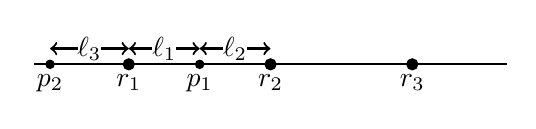
\begin{tikzpicture}
    
        
        \draw[black,thick] (0, 0) -- (6, 0);
        
        \filldraw[black] (0.2, 0) circle (1.5pt)
        node[anchor=north]{$p_2$};
        
        \draw[thick, <-] (0.2, 0.2) -- (0.55, 0.2); 
        \node[] at (0.7,0.2) {$\ell_3$};
        \draw[thick, ->] (0.85, 0.2) -- (1.2, 0.2);
        
        \filldraw[black] (1.2, 0) circle (2pt) node[anchor=north]{$r_1$};
        
        \draw[thick, <-] (1.2, 0.2) -- (1.5, 0.2);
        \node[] at (1.65,0.2) {$\ell_1$};
        \draw[thick, ->] (1.8, 0.2) -- (2.1, 0.2);
        
        \filldraw[black] (2.1, 0) circle (1.5pt)
        node[anchor=north]{$p_1$};
        
        \draw[thick, <-] (2.1, 0.2) -- (2.4, 0.2);
        \node[] at (2.55,0.2) {$\ell_2$};
        \draw[thick, ->] (2.7, 0.2) -- (3, 0.2);
        
        \filldraw[black] (3, 0) circle (2pt) node[anchor=north]{$r_2$};
        
        \filldraw[black] (4.8, 0) circle (2pt) node[anchor=north]{$r_3$};
        
        
    \end{tikzpicture}
    \caption{Illustration of the robot sensing model. The segment is being covered by three robot guards $r_1 \sim r_3$. The coverage probability of $p_1$, falling between robots $r_1$ and $r_2$, is given as $\rho(\ell_1)+\rho(\ell_2)-\rho(\ell_1)\cdot\rho(\ell_2)$, and the coverage probability of $p_2$, covered only by $r_1$ is given as $\rho(\ell_3)$.}
    \label{fig:sensing}
\end{figure}


For covering a line segment with a length of $\ell$ and sensing function of $\rho$, 
we denote as $\zeta: \mathbb{R}^+ \rightarrow \mathbb{N}^+$ a primitive for computing 
the minimum number of robots needed to achieve the required minimum covering 
probability of $\rho_0$. 
%Denote the primitive as $\zeta: \mathbb{R}^+ \rightarrow \mathbb{N}^+$.

Take the exponential decaying sensing probability function as an example, 
where $\rho(r) = e^{-c\cdot r}$, $c>0$ is some constant.
In this case, the maximum distance at the two ends to guarantee the sensing probability of $\rho_0$ is $d_1=-\ln (\rho_0)/c$. 
If a point is between two robots with distance $\ell_1$ and $\ell_2$ to the two robots, its sensing probability is bounded by

\begin{align*}
\rho(\ell_1) + \rho(\ell_2) - \rho(\ell_1)\cdot \rho(\ell_2)\geq 2e^{-\frac{c\cdot d}{2}} - e^{-c\cdot d}    \\
where\ d = \ell_1+\ell_2
\end{align*}

So, the required maximum distance between two neighboring robots is $d_2=-2\ln(1-\sqrt{1-\rho_0})/c$.
Therefore, the minimum number of robots required to cover a line segment with length $\ell$ is 
$\zeta(\ell) = \max(1, 1 + \lceil(\ell-2\cdot d_1)/d_2 \rceil )$.


\subsection{Problem Formulation}
In this paper, we work with a 2D compact (i.e., closed and bounded) workspace 
${\mathcal W} \subset \mathbb{R}^2$, which can contain a set of obstacles. 
An existing \emph{sweep schedule} is an input to the problem, which we
define the \emph{continuous monotone sweep schedule} for $\mathcal W$ as 
\begin{definition}[Continuous Monotone Sweep Schedule]
A function $P(t)$ that maps a positive timestamp $t$ to a continuous curve is a continuous monotone sweep schedule for $\mathcal W$ if $P(t)$ changes continuously, 
and for each point $p\in \mathcal W$, there exists a single $t'$ such that $p\in P(t')$.
\end{definition}

Intuitively, a continuous monotone sweep schedule defines a function 
that maps the time step to a 1-D curve in the workspace that sweeps 
through each point in $\mathcal W$ only once. 
%
Depending on the continuous curve, $P(t)$ could take various forms. For example, the sweep line may be straight in a search-and-rescue scenario. Or the sweep line may be circular in a search-and-capture scenario. 
%e a  
%vertical sweeping, circular shrinking, and so on. 
In the rest of this paper, we simply refer to a continuous monotone sweep schedule as a \emph{sweep schedule}. Next, we introduce the notions of \emph{arrival time} and \emph{monotone chain}.
%
\begin{definition}[Arrival Time]
For a search schedule $P(t)$, and a point in the workspace $o\in\mathcal W$,
the arrival time at $o$, $arrival(o)$, is defined as the time step $t$ when $o\in P(t)$.
\end{definition}

\begin{definition}[Monotone Chain]
For a bounded 2D chain: $\tau(s): [0,1]\rightarrow\mathcal{W}$, where $\tau$ is a continuous function, it is considered as a monotone chain to the search schedule $P(t)$ if and only if
\[s_1 < s_2 \Leftrightarrow arrival(\tau(s_1)) < arrival(\tau(s_2)).\]
\end{definition}
In a search schedule or plan, $P(t)$ may be intersected by obstacles. In this case, $P(t)$ is separated into multiple continuous segments; each of these segments requires a dedicated group of robots. That is, robots on one continuous segment cannot provide coverage of other segments. 

%\r{We may want to define the classes of $\mathcal W$ that we work with. We want to work on a class of environment than can be swept with scan lines. This means that the non-convex obstacles must be able to ``see'' the outside in a some sense.}

With the probabilistic robot sensing model, we formulate the robot team scheduling problem for a given sweep schedule as the following,
\begin{problem}
Given a sweep schedule $P(t)$ for a 2D region $\mathcal W$, and a group of robots with coverage capability function $\rho$, what is the minimum number of robots required to execute the sweep schedule on the sweep line, such that 
for every point $o$ in $\mathcal W$, the probability that $o$ is covered is at 
least some fixed $0 < \rho_0 \le 1$?
\end{problem}



\subsection{Optimal Robot Allocation}

% \newcommand{\bdag}{{\textsc DAG}}

Our proposed algorithm can be divided into two steps at the high level. 
In the first step, the algorithm conducts a \emph{generalized boustrophedon 
decomposition} for the given environment along the sweep line, 
which generates a \textit{directed acyclic graph} (DAG) representation 
of the workspace $\mathcal W$ for a given sweep schedule. 
Using the DAG, a max-flow-based algorithm is then applied to compute the 
minimum number of robots required for executing the sweep schedule, 
as well as the corresponding arrangement of robots.

\subsection{Generalized Boustrophedon Decomposition}
In solving search and coverage problems, various decomposition techniques 
have been proposed, including trapezoidal, Voronoi, boustrophedon, Morse decompositions, 
and so on \cite{huang2001optimal, choset2000coverage, breitenmoser2010voronoi, acar2002morse}.
For our robot allocation task, it is also natural to start with a decomposition 
of the environment. 
However, we need a decomposition supporting non-straight 
boundaries between the decomposed cells, created by the sweep schedule. 
For this, we propose a generalization of boustrophedon decomposition. 

Before describing the generalization of boustrophedon decomposition, 
we briefly introduce boustrophedon decomposition (readers are referred to 
\cite{choset2000coverage} for further details), which in turn is based on 
trapezoidal decomposition. The difference is that it removes the sweeping 
events that cross inner vertices. As illustrated in ~\ref{fig:sc-trebou},
compared with trapezoidal decomposition, boustrophedon decomposition 
has fewer cells, which leads to fewer (back-and-forth) boustrophedon motions.

\begin{figure}[ht]
    \centering
    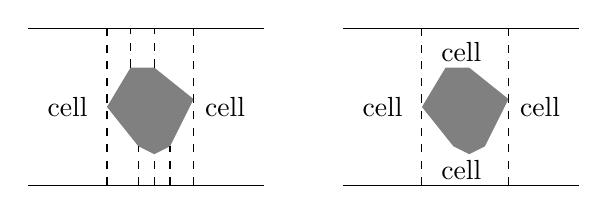
\begin{tikzpicture}
    % \fill[black] (0, 0) -- (1.9, 0.1) -- (1.3, 1) -- (1.85, 1.6) -- (0.1, 1.6) -- (0.7, 0.9) -- cycle;
    \fill[gray] (0, 0) -- (0.4, -0.5) -- (0.6, -0.6) -- (0.8, -0.5) -- (1.1, 0.1) -- (0.6, 0.5) -- (0.3, 0.5) -- cycle;
    \draw (-1, - 1) -- (2, -1); 
    \draw (-1, 1) -- (2, 1); 
    \draw[dashed] (0, -1) -- (0,1);
    \draw[dashed] (0.4, -1) -- (0.4,-0.5);
    \draw[dashed] (0.6, -1) -- (0.6,-.6);
    \draw[dashed] (0.8, -1) -- (0.8,-0.5);
    \draw[dashed] (1.1, -1) -- (1.1,1);
    \draw[dashed] (0.6, 0.5) -- (0.6,1);
    \draw[dashed] (0.3, 0.5) -- (0.3,1);
    
    \node[text=black] at (-0.5, 0.0) {cell};
    \node[text=black] at (1.5, 0.0) {cell};
    
    \fill[gray] (4, 0) -- (4.4, -0.5) -- (4.6, -0.6) -- (4.8, -0.5) -- (5.1, 0.1) -- (4.6, 0.5) -- (4.3, 0.5) -- cycle;
    
    \draw (3, - 1) -- (6, -1); 
    \draw (3, 1) -- (6, 1); 
    
    \draw[dashed] (4, -1) -- (4, 1);
    \draw[dashed] (5.1, -1) -- (5.1, 1);
    
    
    \node[text=black] at (3.5, 0.0) {cell};
    \node[text=black] at (4.5, -.8) {cell};
    \node[text=black] at (4.5, 0.7) {cell};
    \node[text=black] at (5.5, 0.0) {cell};

    \end{tikzpicture}
    \caption{[left] A trapezoidal decomposition, creating a total of $9$ cells. [right]
    Boustrophedon decomposition of the same environment, creating only $4$ cells.}
    \label{fig:sc-trebou}
\end{figure}

We extend the boustrophedon decomposition from using only vertical sweep lines 
to allow the use of any \emph{continuous monotone sweep schedule}.
We are given a sweep schedule $P(t)$ for a workspace $\mathcal W$, 
which could take any curved form (see ~\ref{fig:sc-Bou}).
By following the sweep schedule, it is possible to
construct a decomposition of $\mathcal W$, based on the events of cell
splitting and merging. 

\begin{figure}[ht]
    \centering
    % \includegraphics[width = .3\textwidth]{fig/bou.eps}
    \begin{overpic}[width = .4\textwidth]{chapters/sc/fig/genbou.eps}
    \put(8, 35){$v_1$}
    \put(20, 10){$v_2$}
    \put(20, 30){$v_3$}
    \put(36.5, 42){$v_4$}
    \put(55, 20){$v_5$}
    \put(50, 40){$v_6$}
    \put(80, 30){$v_7$}
    \end{overpic}
    \caption{Suppose we have a sweep schedule that sweeps the environment from left 
    to right, with curved sweep fronts. 
    The curves, as they cross critical vertices of objects, are shown as the 
    dashed lines.
    The generalized boustrophedon decomposition decomposes and $\mathcal W$ into 
    $7$ cells, $v_1\sim v_7$. 
    %
    It is important to note here that, for any continuous monotone sweep schedule,
    a decomposition can be obtained. 
    }
    \label{fig:sc-Bou}
\end{figure}


\begin{theorem}
A sweep schedule can be organized in a DAG by the generalized boustrophedon decomposition.
\end{theorem}

\begin{proof}
Following the sweep schedule, we can conduct a generalized boustrophedon 
decomposition of the workspace $\mathcal W$. 
%
A node in the DAG will represent a cell after the decomposition, whose 
parents and children are the predecessor and successor cells along the 
sweep schedule. 

Additionally, we add a source node that links to all nodes without a parent 
and add a terminal node that links from all nodes without a child.
%
Since obstacles in the environment can contain concave vertices, we must 
consider two special cases involving concave vertices for the construction of DAG, 
as illustrated in ~\ref{fig:sc-concave_vertices}. 
%
When a line segment of the sweep schedule ends at a concave vertex, 
the corresponding node in the DAG is linked to the terminal node $t$.
When a line segment of the sweep schedule starts at a concave vertex,
the corresponding node in the DAG is linked from the source node $s$.
In mapping these scenarios to detailed plans, it means that 
some robots will start later or end earlier compared with 
others.
% \end{remark}

\begin{figure} [ht]
    \centering
    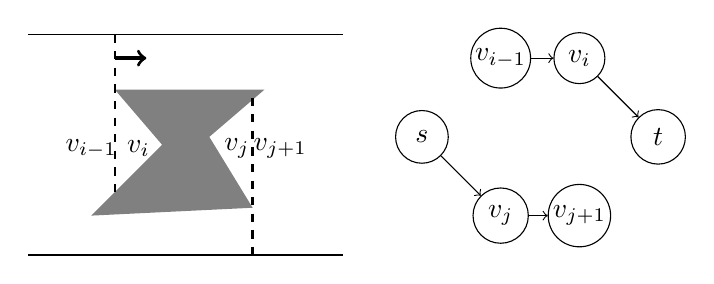
\begin{tikzpicture}
    \fill[gray] (-0.2, 0) -- (1.85, 0.1) -- (1.3, 1) -- (2.0, 1.6) -- (0.1, 1.6) -- (0.7, 0.9) -- cycle;
    \draw (-1, - 0.5) -- (3, -.5); 
    \draw (-1, 2.3) -- (3, 2.3); 

    \draw[dashed, line width=0.9pt, black] (0.1, 2.3) -- (0.1, 0.3);
    \draw[dashed, line width=0.9pt, black] (1.85, 1.5) -- (1.85, -0.5);
    
    
    \draw(-0.2, 0.85) node[text=black] { $v_{i\text{-}1}$};
    \draw(0.4, 0.85) node[text=black] {$v_i$};
    \node[text=black] at (1.65, 0.85) {$v_j$};
    \node[text=black] at (2.2, 0.85) {$v_{j\text{+}1}$};
    
    \draw(4, 1.0) node [circle, radius = 0.12, draw, inner sep=4.5](s){ $s$};
    
    \draw(5, 2.0) node [circle, radius = 0.12, draw, inner sep=0.8](vi1){ $v_{i\text{-}1}$};
    \draw(6, 2.0) node [circle, radius = 0.12, draw, inner sep=3](vi){ $v_{i}$};
    
    \draw(5, 0.0) node [circle, radius = 0.12, draw, inner sep=3](vj){ $v_{j}$};
    \draw(6, 0.0) node [circle, radius = 0.12, draw, inner sep=0.8](vj1){ $v_{j\text{+}1}$};
    
    \draw(7, 1.0) node [circle, radius = 0.12, draw, inner sep=4.5](t){ $t$};
    
    \draw[->] (vi) -- (t);
    \draw[->] (vi1) -- (vi);
    
    \draw[->] (vj) -- (vj1);
    \draw[->] (s) -- (vj);
    
    \draw[very thick, ->] (0.1, 2.0) -- (0.5,2.0);
    \end{tikzpicture}
    \caption{An example that contains two concave scenarios. As a result of the DAG construction, some robots will
    start their work at $v_j$ (by having $s$ as its parent) and some robots will end their work at $v_i$ (by having $t$ as its child).}
    \label{fig:sc-concave_vertices}
\end{figure}
\end{proof}

% \begin{remark}



The implementation of the generalized boustrophedon decomposition is similar 
to vertical decomposition, we provide here an implementation 
Alg.~\ref{alg:genbou} adapted from \cite{lavalle2006sweepline} under the 
\emph{generation position} assumption (i.e., there are no degenerative 
settings).
%
Basically, the algorithm works by maintaining a binary search tree for 
\emph{boundary chains} representing cell boundaries. The algorithm considers 
two types of events during the sweeping process: splitting a cell into two 
cells and merging two cells into one cell.
%
Since the time cost mainly comes from maintaining the binary search tree of 
chains, with an efficient implementation, Alg.~\ref{alg:genbou} requires 
$O(n \log n)$ time, where $n$ is the complexity of the environment. 


\subsection{Reduction to Circulation with Demand}
Since we are working with \emph{monotone sweep schedules}, for any point $p$ in 
$\mathcal W$, it can only be contained in $P(t')$ for a single $t'$, i.e., each 
point $p \in \mathcal W$ is only swept once. 
%
Denote the length of the line segment where it is contained as $L$, which 
requires at least $\zeta(L)$ robots inside that segment at time $t'$
(recall that $\zeta$ is the primitive defined in Sec.~\ref{sec:sc-sensing}).
%
For each decomposed cell, the minimum number of robots required is $\zeta(\ell_{max})$, where $\ell_{max}$ 
is the maximum length of the sweep line inside that cell.
%
Given a DAG $G(V,E)$ that represents the sweep schedule, the arrangement problem of the robots along the sweep line can be transformed into a network 
flow problem on the DAG.
%
For each node $v\in G$, there is a requirement of coverage for the node, 
$demand(v)$, which can be computed as $\zeta(v.\ell_{max})$.
%
Given the DAG and the demands, we are then to ``flow'' the robots through 
the schedule, allocating a certain number of robots to each decomposed cell 
along the way to satisfy these demands. 
%

Specifically, our problem may be further cast as a \emph{circulation with demand} 
problem \cite{kleinberg2006algorithm}, with the following augmentation. We replace 
each node $v$ in $G$ with two vertices $v_1$ and $v_2$ and replace every edge 
$uv$ in the previous graph with edge $u_2 v_1$, as illustrated in ~\ref{fig:sc-flow}. 
The edge between $v_1$ and $v_2$ has flow demand of $demand(v)$. 
The following minimum circulation with demand problem is then obtained.

\begin{algorithm}[h!]
\SetKwFunction{genbou}{GenBouDecomp}
%\begin{small}
\KwData{$P(t)$: a sweep schedule. $\mathcal W$: the workspace.}
\KwResult{a DAG from the decomposition.}
\vspace{1mm}
\SetKwComment{comment}{\%}{}
\DontPrintSemicolon
\SetKw{arrival}{Arrival}

1. Separate the boundaries of obstacles into a set of \emph{monotone chains},
where each chain has the points on it \emph{arrival time} arranged in an 
increasing order.;\;
\vspace{0.5mm}
% Denote $k$ as the number of chains obtains;\;

2. $T\gets$ A binary search  tree of the chains\;
\vspace{0.5mm}

3. Construct an \emph{event array} that contains the events of the start of a chain and the end of a chain, sorted by their occurrence time during the sweep.\;
\vspace{0.5mm}

4. Iterate over the event array, which inserts and deletes chains from the binary search tree $T$, while making sure that $T$ represents the current order of the chains.\;
\vspace{0.5mm}
%\comment{\begin{footnotesize}With the general position assumption, the events comes as a paired operation for either deletion or insertion of chains \end{footnotesize}}

% When two chains are added to $T$, a cell is split into two new cells in the case of convex
% vertex or a new cell is created.  An edge from $s$ is added for a concave vertex.\;
When two chains are added to $T$, a cell is split into two new cells in the case of a convex vertex, or a new cell is created for a concave vertex, where an edge directed from $s$ is added.\;
% When two chains are removed from $T$, two cells are merged into a new cell in the case of 
% convex vertex or a cell disappears. An edge is added to $t$ for a concave vertex.\;
When two chains are removed from $T$, two cells are merged into a new cell in the case of a convex vertex or a cell disappears for a concave vertex, where an edge is added directed to $t$.\;

5. Return the DAG constructed based on $P(t)$.
%\end{small}
\caption{\protect\genbou{$P$, $\mathcal{W}$}: Generalized Boustrophedon Decomposition} 
\label{alg:genbou}
\end{algorithm}

\begin{figure}[h]
    \centering
    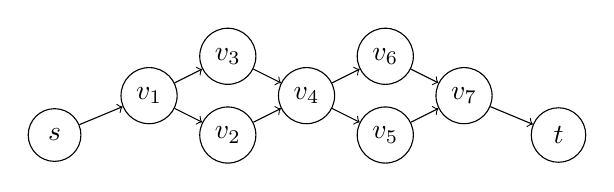
\begin{tikzpicture}
    % \node[circle](v1){$v1$};
    % \node[circle](v2){$v2$};
    % \draw[->] (v1.east) -- (v2.west);
    \draw(0,0) node [circle, radius = 0.12, draw](v1){ $v_1$};
    \draw(1, -0.5) node [circle, radius = 0.12, draw](v2){ $v_2$};
    \draw(1, 0.5) node [circle, radius = 0.12, draw](v3){ $v_3$};
    \draw(2, 0.0) node [circle, radius = 0.12, draw](v4){ $v_4$};
    \draw(3, -0.5) node [circle, radius = 0.12, draw](v5){ $v_5$};
    \draw(3, 0.5) node [circle, radius = 0.12, draw](v6){ $v_6$};
    \draw(4, 0.0) node [circle, radius = 0.12, draw](v7){ $v_7$};
    
    \draw(-1.2, -.5) node [circle, radius = 0.2, draw,inner sep=4.5](s){ $s$};
    
    \draw(5.2, -.5) node [circle, radius = 0.2, draw,inner sep=4.5](t){ $t$};
    
    \draw[->] (v1) -- (v2);
    \draw[->] (v1) -- (v3);
    \draw[->] (v2) -- (v4);
    \draw[->] (v3) -- (v4);
    \draw[->] (v4) -- (v5);
    \draw[->] (v4) -- (v6);
    \draw[->] (v5) -- (v7);
    \draw[->] (v6) -- (v7);
    
    \draw[->] (s) -- (v1);
    \draw[->] (v7) -- (t);
    \end{tikzpicture}
    \caption{The constructed DAG from the example in ~\ref{fig:sc-Bou}}
    \label{fig:sc-DAG}
\end{figure}


\begin{algorithm}[h!]
%\begin{small}
\DontPrintSemicolon
\SetKwFunction{mindag}{MinSweepDAG}
\SetKwFunction{dflow}{MinCirculationWithDemand}
\SetKwFunction{addedge}{add\_edge}
\SetKwFunction{addvertex}{add\_vertex}
\KwData{$dag(V, E)$: the DAG obtained from \genbou. $\zeta$: the sensing requirement primitive function.}
\KwResult{$dag$: the updated $dag$ with the robot allocation information}
\vspace{0.5mm}
$G'\gets$ a new empty graph;\;
\vspace{0.5mm}

\For{$v\in dag$}{
\vspace{0.5mm}
    $G'$.\addvertex$(v_1),$ $ G'$.\addvertex($v_2$);\;
\vspace{0.5mm}
    
    $G'.$\addedge($v_1, v2$, capa=$\infty$, demand=$\zeta(v.\ell_{max})$);\;
\vspace{0.5mm}
    
    \For{$u\in dag.neighbor[v]$}{
\vspace{0.5mm}
        $G'$.\addedge($v_2$, $u$, capa=$\infty$, demand=0);\;
    }
}
\vspace{0.5mm}

\dflow($G'$);\;
\vspace{0.5mm}

\For{$v\in dag$}{
\vspace{0.5mm}
    $dag.v.guards\_num\gets$ $G'.flow[v_1][v_2]$;\;
    
\vspace{0.5mm}
    \For{$u\in dag.neighbor[v]$}{
        $dag.flow[v][u] = G'.flow[v_2][u_1]$;\;
    }
    
}


\Return{$dag$}\;

% \begin{small}

%\end{small}
\caption{\protect\mindag{$dag$, $\zeta$}{}}
\label{alg:mindag}
\end{algorithm}

\begin{figure*}[h!]
\vspace{2mm}
    \centering
    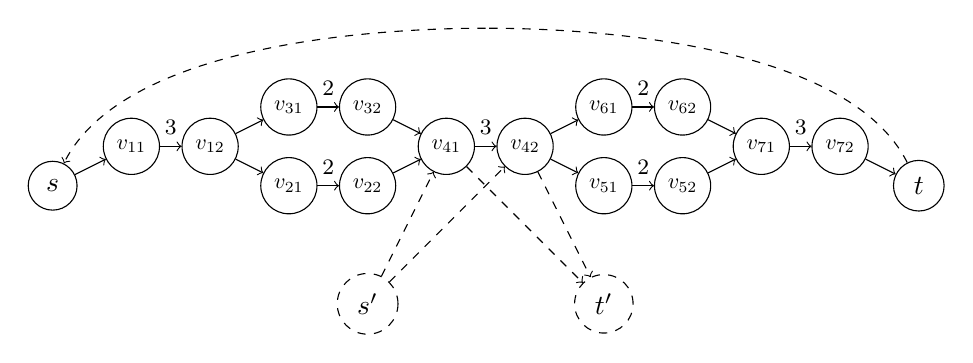
\begin{tikzpicture}[scale = 1, every node/.style={inner sep=4}]
    \draw(0,0) node [circle, draw, scale = 0.8](v11){ $v_{11}$};
    \draw(1,0) node [circle, draw, scale = 0.8](v12){ $v_{12}$};
    
    \draw(2, -0.5) node [circle, draw, scale = 0.8](v21){ $v_{21}$};
    \draw(3, -0.5) node [circle, draw, scale = 0.8](v22){ $v_{22}$};
    
    \draw(2, 0.5) node [circle, draw, scale = 0.8](v31){ $v_{31}$};
    \draw(3, 0.5) node [circle, draw, scale = 0.8](v32){ $v_{32}$};
    
    \draw(4, 0.0) node [circle, draw, scale = 0.8](v41){ $v_{41}$};
    \draw(5, 0.0) node [circle, draw, scale = 0.8](v42){ $v_{42}$};
    
    \draw(6, -0.5) node [circle, draw, scale = 0.8](v51){ $v_{51}$};
    \draw(7, -0.5) node [circle, draw, scale = 0.8](v52){ $v_{52}$};
    
    \draw(6, 0.5) node [circle, draw, scale = 0.8](v61){ $v_{61}$};
    \draw(7, 0.5) node [circle, draw, scale = 0.8](v62){ $v_{62}$};
    
    \draw(8, 0.0) node [circle, draw, scale = 0.8](v71){ $v_{71}$};
    \draw(9, 0.0) node [circle, draw, scale = 0.8](v72){ $v_{72}$};
    
    \draw(-1, -.5) node [circle, draw](s){ $s$};
    \draw(10, -.5) node [circle, draw](t){ $t$};
    
    \draw[->] (v12) -- (v21);
    \draw[->] (v12) -- (v31);
    \draw[->] (v22) -- (v41);
    \draw[->] (v32) -- (v41);
    \draw[->] (v42) -- (v51);
    \draw[->] (v42) -- (v61);
    \draw[->] (v52) -- (v71);
    \draw[->] (v62) -- (v71);
    
    \draw[->] (v11) -- node[above]{\footnotesize $3$} (v12) ;
    \draw[->] (v21) -- node[above]{\footnotesize $2$} (v22) ;
    \draw[->] (v31) -- node[above]{\footnotesize $2$} (v32) ;
    \draw[->] (v41) -- node[above]{\footnotesize $3$} (v42) ;
    \draw[->] (v51) -- node[above]{\footnotesize $2$} (v52) ;
    \draw[->] (v61) -- node[above]{\footnotesize $2$} (v62) ;
    \draw[->] (v71) -- node[above]{\footnotesize $3$} (v72) ;
    
    \draw[->] (s) -- (v11) ;
    \draw[->] (v72) -- (t) ;
    
    \draw[dashed] (t) .. controls(9, 1.5) and (5, 1.5) .. (4.5, 1.5);
    \draw[dashed,->] (4.5,1.5) .. controls(4,1.5) and (0,1.5) .. (s);
    
    \draw(3, -2) node [circle, draw, dashed] (s'){$s'$};
    \draw(6, -2) node [circle, draw, dashed] (t'){$t'$};
    
    \draw[dashed,->] (s') -- (v41);
    \draw[dashed,->] (v41) -- (t');
    
    \draw[dashed,->] (s') -- (v42);
    \draw[dashed,->] (v42) --  (t');
    
    \end{tikzpicture}
    \caption{Transform the DAG in ~\ref{fig:sc-DAG} into a circulation with demand problem. 
    The value above each edge represents the demand of the edge, which is eliminated when it is zero.
    The source node is $s$, and the target node is $t$. $s'$ and $t'$ are the auxiliary source and target for solving the ``circulation with demand'' problem.
    Also, auxiliary edges are added between $s', t'$ and every other vertex.}
    \label{fig:sc-flow}
\end{figure*}


\begin{problem}[Minimum Circulation with Demand]
There is a graph $G(V,E)$, where $s,t$ are the source and terminal nodes. 
Every edge $uv$ in $G$ has a demand of $d(uv)$ and a capacity of $c(uv)$. 
Compute minimal network flow from $s$ to $t$ that saturates all the edge 
demands.
\end{problem}

Readers are referred to \cite{kleinberg2006algorithm} for %detailed algorithm   description and proof of correctness 
the details of the classical ``circulation with demand'' problem solution with max-flow. 

Alg.~\ref{alg:mindag} outlines the operations
used in this section. We note that the 
graph data structure needs to have the functionality of adding vertex and adding 
edge with edge demand, and $G'.flow[v_1][v_2]$ denotes the flow from $v_1$ to $v_2$ on $G'$.
% By solving the maxflow problem, we 

\subsection{The Complete Allocation Algorithm}
The overall algorithm for robot allocation is described as in Alg.~\ref{alg:sc-overall}.
To analyze the running time of Alg.~\ref{alg:sc-overall} for a polygonal environment, 
we denote the environment complexity (number of vertices) as $n$. 
As mentioned in the previous section, the generalized boustrophedon decomposition takes $O(n\log n)$ time. 
As the generation of a node in the DAG comes from some chain insertion or deletion events, and an event would require one vertex to happen, 
there is at most $O(n)$ decomposed cells, i.e., nodes in the DAG. 
Similarly, adding edges between nodes comes from some chain insertion or deletion events, and the number of events is at most $O(n)$. 
So, both the number of edges and the number of nodes in the DAG is $O(n)$.
Moreover, it is easy to see that the DAG is a planar graph since a node corresponds to a decomposed cell, and there is an edge between nodes only if the two corresponding cells are adjacent.
The circulation with demand problem requires solving two max-flow problems based on the DAG. 
If we use the push-relabel algorithm \cite{cheriyan1989analysis} that runs in $O(V^2\sqrt{E})$, solving the max flow for this problem will cost $O(n^{2.5})$, 
% If we use the Dinic's algorithm \cite{dinitz1970algorithm} that runs in $O(V^2E)$, solving the max flow for this problem will cost $O(n^{3})$, 
since $|V|, |E| = O(n)$.% for planar graphs. 

\begin{algorithm}[ht]
%\begin{small}
\SetKwFunction{minsweep}{MinSweep}
\KwData{$P(t)$: a sweep schedule. $\mathcal W$: a compact workspace.
$\rho_0$: required sensing probability guarantee.
% Primitive function $\zeta$ to compute the minimum number of line guards required for a continuous line segment.
}
\KwResult{$n$: the minimum number of robot guards required. $plan$: the corresponding allocation plan}%, embedded in a DAG.}
\SetKwComment{comment}{\%}{}

\vspace{1mm}
Construct $\zeta$ based the sensing model and $\rho_0$\;
\vspace{1mm}

\begin{small}
\comment{Primitive function $\zeta$ is to compute the minimum number of robots required for a continuous line segment}
\end{small}
\vspace{1mm}
$dag\leftarrow \genbou(P, {\mathcal W})$;\;

\vspace{1mm}
$dag\gets \mindag(dag, \zeta)$;\;

\vspace{1mm}
$plan\gets dag$;\;

\vspace{1mm}
\begin{small}
\comment{The plan of the robots can be constructed based on the flow on the $dag$.} 
\end{small}

\vspace{1mm}
\Return{$dag.s.guards\_num$, plan};\;
% Step 2. Construct corresponding DAG for the robot sweep schedule, as well as 
% the minimum number of robots required: $\zeta(\ell_m)$ for each cell\;

% Step 3. Run the minimum flow with demand algorithm on the transformed DAG, which results in the allocation of the robots\;
%\end{small}
\caption{\protect\minsweep{$P, {\mathcal{W}}, \rho_0$}: Computing Minimum Number of Robots for a Sweep Schedule}
\label{alg:sc-overall}
\end{algorithm}



\begin{remark}
In the case of having a fixed number of robots, 
and the objective is to 
maximize the minimum coverage probability of a point in $\mathcal W$.
We can apply binary search on the minimum coverage probability we can guarantee, 
where Alg.~\ref{alg:sc-overall} can be used to decide whether some coverage probability can be guaranteed by 
the fixed number of robots.
% The algorithm is detailed out in Alg.~\ref{alg:fixednum}
%\r{I think a remark is enough to say it}
\end{remark}

% \begin{algorithm}[ht]
% \begin{small}
% \SetKwFunction{maxprob}{MaxProb}
% \KwData{ $P(t)$: a sweep schedule. 
% $\mathcal W:$ a compact workspace.  $k$: the number of robots. }
% \KwResult{an allocation plan for $k$ robots to achieve 
% maximum guaranteed coverage probability, embedded in a DAG.}

% $\rho_{min}, \rho_{max}\leftarrow  0$, $1$;\;

% \While{$\rho_{max}-\rho_{min} \geq \varepsilon$}{
%     % \State Construct $\zeta$ based on $\rho_{mid}=(\rho_{min} + \rho_{max})/{2}$\\
%      $n$, $plan$ $\gets \minsweep(P, {\mathcal W}, \rho_{min})$;\;
    
%     \eIf{$n > k$}{
%          $\rho_{max} \gets \rho_{mid}$;\;
%     }{
%          $\rho_{min} \gets \rho_{mid}$;\;
%     }

% }
% \Return{$\rho_{min}$, plan}
% \end{small}
% \caption{\maxprob$(P, \mathcal{W}, k)$: Maximizing the Sensing Probability Guarantee for a Sweep Schedule with Fixed Number of Robots }
% \label{alg:fixednum}
% \end{algorithm}


\subsection{Simulation Evaluation}
In this section, we perform a numerical evaluation of our proposed method
with two goals: (1) confirms the scalability and (2) observe the behavior 
of the method as input parameters change. 
%
We implemented our proposed algorithms in C++. Dinic's algorithm is used to solve the max-flow problem \cite{dinitz1970algorithm} for simplicity. 
The methods are evaluated at an Intel\textsuperscript{\textregistered} Core\textsuperscript{TM} i5-10600K CPU at 4.1HZ.
%
For the three use cases (~\ref{fig:sc-sweep} (b)(c)(d)), we
programmatically create a large number of test cases, with up to 
$6,000$ randomly generated polygonal obstacles. 
%
The number of vertices of each polygon ranges from 3 to 50, making the total vertices up to 
$100,000+$. 
%
~\ref{fig:sc-cases} shows the largest problem instances for the experiments with 
around $100,000$ vertices.
\begin{figure}[ht]
    \centering
    \includegraphics[width=.95\linewidth]{chapters/sc/fig/cases.png}
    \caption{Examples of programmatically generated test environments with total 
    vertices around $100,000$.}
    \label{fig:sc-cases}
\end{figure}

\textbf{Algorithm performance.} In a first set of evaluations, under an exponentially 
decaying sensing 
model, $\rho(r) = e^{-c\cdot r}$, we test the performance of our algorithm over 
the set of instances. Example allocation of robots along the sweep frontiers for 
the three cases are shown in ~\ref{fig:sc-sweep}(a) and ~\ref{fig:sc-simulations}. 
We limited the number of robots to be small so that the trajectories are more easily 
observed. It can be seen that the trajectories can vary significantly along the 
sweep frontiers for each case. 
% The first setting uses vertical sweep as the search schedule to sweep a rectangle.
% The second setting uses circular sweep, where guards are tasked to
% sweep $\mathcal{W}$ in a circular expansion manner.
% The thirst setting uses radial expansion as the search schedule, that is 
% a group of guards are tasked to sweep a circular regions in a radial rotational manner.
\begin{figure}[ht]
    \centering
    % 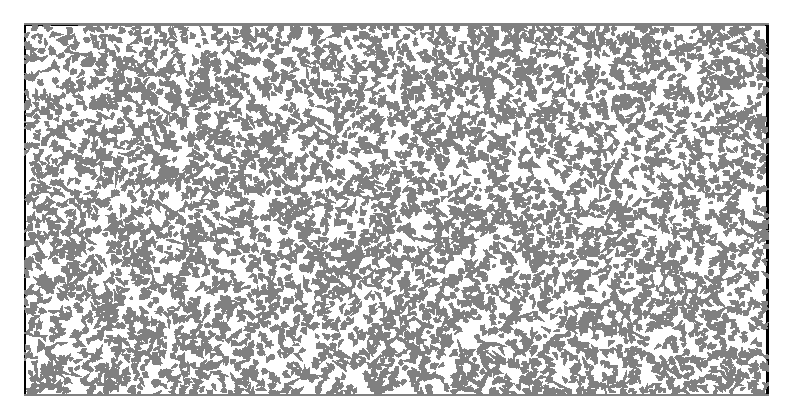
\includegraphics[width=.45\linewidth]{fig/vertical_large.eps}
    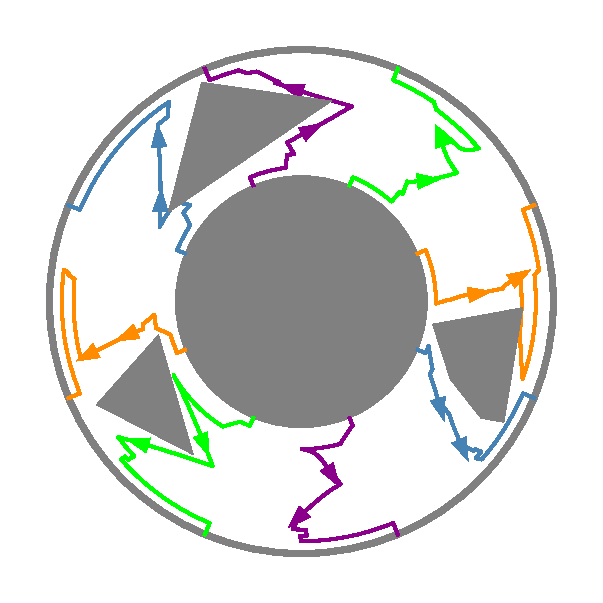
\includegraphics[width=.45\linewidth]{chapters/sc/fig/circular_sol.eps}\hspace{2mm}
    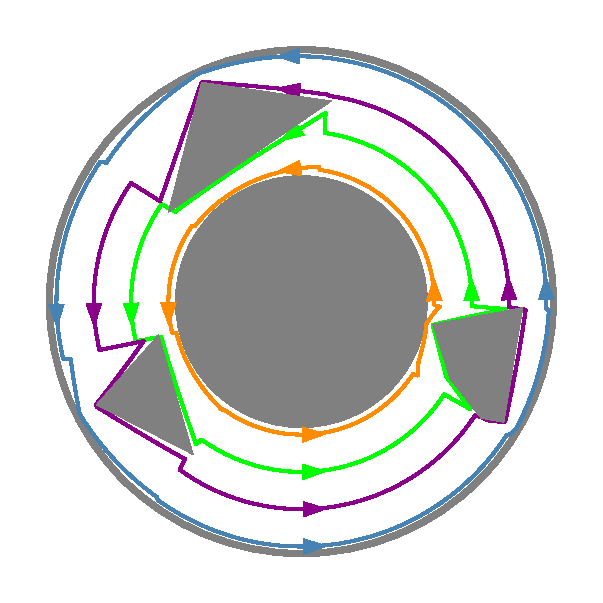
\includegraphics[width=.45\linewidth]{chapters/sc/fig/rotational_sol.eps}
    
    \caption[Example robot trajectories]{Example robot trajectories computed by our method for circular and radial 
    sweep use cases, respectively.
    }
    \label{fig:sc-simulations}
\end{figure}

In ~\ref{fig:sc-simulations_runtime}, the computational performance is thoroughly 
evaluated. As can be observed, our method scales fairly well, taking less than two seconds
to handle all cases, even those involving over $100,000$ vertices. 
%
%We show the running time information in ~\ref{fig:simulations_runtime}. 
%The algorithm scale up reasonably to $10^5$ vertices in around $1.5s$ for the three sweep patterns. 
Interestingly, the experimental running time is almost linear, even using the less efficient Dinic's algorithm. 
%
We suspect the near linear running time is due to the fact that the DAG is 
a planar graph; studies show that max-flow for planar graphs can be computed 
in $O(n\log n)$ \cite{borradaile2009n}. 
%
Although the graph constructed when solving the ``circulation with demand'' problem is not planar, large portions are planar. 
This could reduce the actual time complexity of running the max-flow algorithm.

\begin{figure}[h]
\vspace{2mm}
    \centering
    \includegraphics[width=0.5\linewidth]{chapters/sc/fig/runtime.eps}
    \caption{Running time in seconds with respect to environment complexity (number of vertices). }
    \label{fig:sc-simulations_runtime}
\end{figure}

\textbf{Different environment settings.}
Lastly, we evaluate the impact of environmental changes, considering factors including the spatial distribution of polygonal obstacles as well as 
the size distribution of the obstacles. 
%
All in all, three settings are considered: (1) The polygons are regularly distributed 
and are of similar size, (2) the polygons are randomly distributed and are of similar size,
and (3) the polygons are regularly distributed, and their sizes can vary dramatically. 
The first and the third settings are illustrated in the top row of ~\ref{fig:sc-runtime_env}.
%
For these settings, we compare the time it takes to compute solutions for many polygonal
obstacles and also the number of robots required to achieve $80\%$ probabilistic guarantee 
under the exponential decay sensing model.
%
As we can observe, there is little difference as the settings change. 

\begin{figure}[h]
    \centering
    \hspace{5mm}
    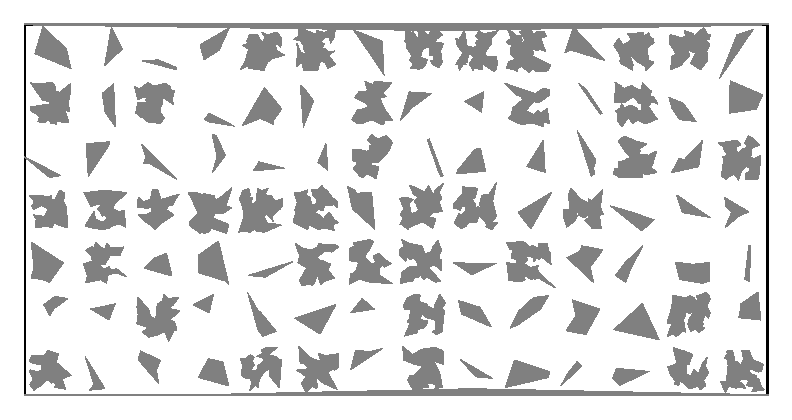
\includegraphics[width = 0.44\linewidth]{chapters/sc/fig/expr_inst_regular.eps}\hspace{1mm}
    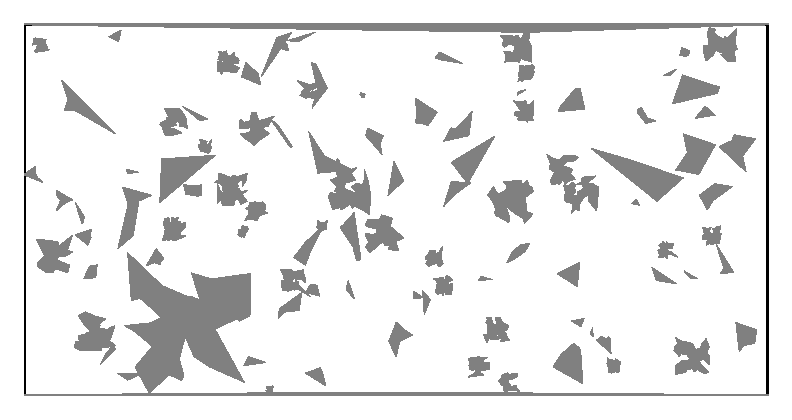
\includegraphics[width = 0.44\linewidth]{chapters/sc/fig/expr_inst_varscale.eps}
    \vspace{3mm}
    
    \includegraphics[width=.47\linewidth]{chapters/sc/fig/runtime_env.eps}
    \includegraphics[width=.48\linewidth]{chapters/sc/fig/n_env.eps}
    \caption[Random instance and runtime time]{
    [top] Random instance with regularly distributed obstacles and instance with random obstacle scales and positions.
    [bottom] Running time for different randomly generated environments and the number of robots required for different randomly generated environments.}
    \label{fig:sc-runtime_env}
\end{figure}

%Based on the evaluation, one somewhat interesting conclusion we can draw is 
%that, the solution to the robot allocation task for carrying out pre-determined 
%sweep schedule is fairly ``stable''; it is unlikely to have dramatic 
\subsection{Conclusion }%\& Future work}

In this section, we studied the problem of allocating a minimum number of robots for a sweep schedule with a probabilistic line sensing model, where a desired level of scanning quality can be guaranteed. 
Towards this, a novel decomposition technique is proposed that generalizes the well-known boustrophedon decomposition. The decomposition leads naturally to a transformation of the problem into a network-flow problem. Due to the decomposition and the transformation, our proposed algorithm runs in low polynomial time and even near $\Tilde{O}(n)$ in simulation experiments for polygonal environments, where $n$ is the complexity of the environment, measured as the number of vertices of polygons. Extensive simulation-based evaluation corroborates the effectiveness of our algorithm, which is applicable to multiple types of environments.  

% In future work, we would like to take the current study in several directions. 
% One further step is to overcome the discontinuities in the robot paths generated. 
% As can be seen in the example trajectory of the robots, 
% when the sweep line crosses vertices, there exists position ``jumps'', though these jumps are transitions inside the sweep line and does not cross objects.
% Intuitively, this requires the sweep line to stop at that position until the robot moved to the next point, or the robot is much faster than the sweep line.
% A second direction is the adaptation to more versatile sweeping plan.
% This work limits the robot to stay on the given search frontier;
% it will be more natural to allow robots to shortly leave the search frontier, e.g., possibly going into or out of a concave region.




\section{Boundary Defense}
\def\prob{{\texttt{{BDHD}}}\xspace}
\def\ours{{{{EDP}}}\xspace}
\def\oours{{{{OEDP}}}\xspace}
\subsection{Introduction}
\subsection{Introduction}

Searching for a static or moving target in a planar environment is a classic 
problem in robotics \cite{guibas1999visibility, suzuki1992searching, lavalle2000algorithm, stiffler2017persistent, kolling2007graph}. 
%
The setting applies to many real-world applications, including searching for
lost person/object, checking for potential hazards, and generally, search and rescue tasks conducted in a known environment. 
%
Research tackling this problem mostly focuses on devising a search plan with
different types of objectives, such as minimizing the total length of the
frontier of the search schedule from the start to the end 
\cite{kolling2017coordinated}, minimizing the number of robots used for 
the search plan in a visibility-based robot sensing model
\cite{megiddo1988complexity}, and so on.

In certain cases, the high-level plan for searching a given region may already be pre-determined and fixed. For example, in search and rescue efforts, a frequently carried out plan is to perform a single sweep of an environment with a marching frontier, which is easy to execute when many participating robots/agents are involved.
%
The high-level search plan may also be determined by existing algorithms that 
compute only the search frontier.
%
However, even in the case where the search plan consists of pre-determined 
sweep (frontier) lines; it remains non-trivial to find an optimal organization 
of the mobile robots to execute the search plan, for either minimizing the 
number of robots needed for a given sensing probability requirement or utilizing 
a fixed number of robots to maximize the minimum sensing probability of locating something in the environment. 

\begin{figure}[t]
\vspace{1.5mm}
    \centering

    \begin{subfigure}[t]{0.7\textwidth}
         \centering
        % \vspace{2.5mm}
         \includegraphics[width=\textwidth]{chapters/sc/fig/instance_2-eps-converted-to.pdf}
        %  \vspace{0.5mm}
         \caption{Optimal robot allocations in a vertical sweep}
         \label{fig:sc-vertical-exp}
     \end{subfigure}
    
    %\includegraphics[width=.475\textwidth]{fig/instance_2-eps-converted-to.pdf}
    \medskip
    
    \begin{subfigure}[t]{0.4\textwidth}
         \centering
        % \vspace{2.5mm}
         \includegraphics[width=\textwidth]{chapters/sc/fig/vertical-eps-converted-to.pdf}
        %  \vspace{0.5mm}
         \caption{Vertical}
         \label{fig:sc-vertical}
     \end{subfigure}
    \begin{subfigure}[t]{0.2\textwidth}
         \centering
         \includegraphics[width=\textwidth]{chapters/sc/fig/circular-eps-converted-to.pdf}
         \caption{Circular}
         \label{fig:sc-radial}
     \end{subfigure}
    \begin{subfigure}[t]{0.2\textwidth}
         \centering
         \includegraphics[width=\textwidth]{chapters/sc/fig/rotational-eps-converted-to.pdf}
         \caption{Radial}
         \label{fig:sc-circular}
    \end{subfigure}
     
    \vspace{2mm}
    \caption[Illustration of sweep schedules]{(a) An illustration of robots' locations along a left-to-right 
    vertical sweep schedule. Four robots are allocated to execute the vertical sweep, 
    and their trajectories are illustrated in different colors. 
    %
    % There exist discontinuities (jumps) along the trajectories when obstacle vertices 
    % intersect the sweep line, induced by topological changes of the environment. 
    (b)(c)(d) Illustrations of three use cases: vertical, circular, 
    and radial sweeps.}
    \label{fig:sc-sweep}
\end{figure}

In this work, we address the challenge of how to best allocate 
many robots to execute a pre-determined search schedule for a known environment. 
More specifically, for a two-dimensional closed and bounded workspace, and a known 
search schedule, which gives a search frontier for any given time, the robot guards 
are required to stay on the search frontier to carry out the sensing task. 
%
Because each robot's coverage quality deteriorates with distance, their relative 
placement on the frontier must be carefully decided to maximize the coverage quality. 
%
For the setup, we focus on the problem of finding the minimum number of robots required 
to execute a pre-determined sweep schedule such that a minimum sensing quality is 
guaranteed for each point in the workspace. Solutions to this minimization problem 
readily translate to solutions for maximizing the coverage quality for a fixed number 
of robots, which is a dual problem. 

In summary, the main contributions of this work are twofold. First, we generalize the 
notion of boustrophedon decomposition \cite{choset2000coverage}, which partitions the 
plane via vertical sweep, into a decomposition of the plane with a \emph{continuous 
monotone sweep schedule}, which we prove can always be represented as a directed 
acyclic graph (DAG). 
%
Then, we show the problem of minimizing the number of line guards required to execute a sweep schedule can be transformed into a network flow problem.
%
Since the generalized boustrophedon decomposition and the network flow problem can 
be solved in low polynomial time; our method achieves high levels of scalability.
%
The strengths of our method are further corroborated in extensive simulation experiments 
on three realistic use cases: \emph{vertical sweep}, \emph{circular sweep}, and 
\emph{radial sweep} (see, e.g., ~\ref{fig:sc-sweep} (b)(c)(d)).





\noindent
% \textbf{Related Work.}
% The study in this paper draws inspiration from the study of several 
% lines of related problems. 
% The Graph-Clear problem, formulated in \cite{kolling2007graph}, tasks a group of robots to search and clear an environment with the operations of blocking and clearing.
% A follow-up work on Line-Clear \cite{kolling2017coordinated} uses line guards
% with more focus on computational geometry in that
% the objective is to minimize the maximum sweep line distance. Both of these problems are
% NP-hard, establishing the difficulties of finding a sweep schedule for a planar environment.
% The more general pursuit-evasion problem dates back to the research on \emph{search number}
% on a discrete graph \cite{megiddo1988complexity}, 
% followed by studies on pursuit and evasion continuous environment with 
% visibility-based model \cite{guibas1999visibility, suzuki1992searching, lavalle2000algorithm, stiffler2017persistent}. 
% The problem becomes the well-known art-gallery problem \cite{o1987art} when a static deployment of robots is sought after.
%
% When working with known patrolling search frontiers, e.g., vertical sweep lines, 
% this problem is analogous to the perimeter defense problem by placing guards on a static perimeter
% to defend intruders \cite{shishika2020cooperative, macharet2020adaptive, chen2021optimal}.
% Previously, we have also studied a version of static range guard placement problems for securing perimeters and regions \cite{fengyu2020optimally}.
% In contrast to the pursuit-evasion algorithms that deal with searching dynamic and unpredictable targets that could escape, 
% coverage planning/control-related algorithms become more suitable for searching or covering predictable or stationary targets,
% e.g., room sweeping, pesticide and fertilizer spraying, persistent monitoring, and so on \cite{cortes2004coverage, oksanen2009coverage, haksar2020spatial, wei2018coverage, deng2019constrained, lan2013planning, cassandras2012optimal, yu2015persistent, palacios2017optimal}. 

\begin{comment}
\noindent
\textbf{Search and rescue}
Graph Clear / Line Clear: 
Andreas Kolling's work like his thesis and some following work as "Coordinated search with multiple robots arranged in line formations" 

\noindent
\textbf{Pursuit evasion}
\noindent
Visibility based: ...

\noindent
\textbf{perimeter defense/guarding}

\noindent
\textbf{Coverage planning}: 
Similar vertical (trapezoidal, boustrophedon) tessellation of plane 

\noindent
"Coverage of Known Spaces: The Boustrophedon Cellular Decomposition"

\noindent
"On Minimizing Turns in Robot Coverage Path Planning"

\noindent
"Coverage Path Planning Algorithms for Agricultural Field Machines"

\noindent
"Optimal Line-sweep-based Decompositions for Coverage Algorithms"



\end{comment}
\label{sec:bd-intro}
\subsection{Preliminaries}\label{sec:bd-preliminary}
In boundary defense with heterogeneous defenders (\prob), there are $k$ defenders (which may be robots and/or other types of agents) with speeds $v_1,\dots,v_k$, where each defender is modeled as a point in some domain $\mathcal E = \mathbb R^2$ or $\mathbb R^3$.
The defenders live on a lower dimensional subspace of $\mathcal E$ (i.e., some boundary of a subset of $\mathcal E$).  
There are also $n$ attack events $\big\langle loc_i, t_i\big\rangle_{i=1}^{n}$, where each attack event is a pair $\big\langle loc, t\big\rangle$ in which $loc$ is the
location of the attack and $t$ is the time it happens. 
The $i^{{th}}$ attack is intercepted by a defender only if the defender is located at $loc_i$ at time $t_i$.
For initialization, we denote the initial locations of the $k$ defenders at $t=0$ as $loc^{1},\dots, loc^{k}$. 

Following the definition in \cite{adler2022role}, we define the horizon of the defenders as follows,
\begin{definition}[Horizon]
The (look ahead) \textit{horizon} $T$ of the defenders is defined as the amount of time defenders can peek into the attack sequence in the future. That is, given the current time $t$, and a horizon $T$, defenders have access to complete information on attacks happening on or before $t+T$. 
\end{definition}

Now, we provide formulations of the two versions of the \prob problem studied in this paper. In the infinite horizon setting, $T = \infty$, all attack events are given in a single batch.

\begin{problem}[Infinite-horizon \prob]\label{prob:1}
Given $k$ defenders with speed $v_1, \dots, v_k$ and initial locations $loc^1, \ldots, loc^k$, and $n$ attack events $\big\langle loc_i, t_i\big\rangle_{i=1}^{n}$, intercept as many attacks as possible. 
\end{problem}

In a finite-horizon setting, the attack events are not all revealed at $t=0$ but are given as a stream of attacks $\big\langle loc_i, t_i\big\rangle_{i=1}^{\infty}$. The defenders can only know the attack events within a horizon or time window of $T < \infty$ in the future.

\begin{problem}[Finite-horizon \prob]\label{prob:2}
There are $k$ defenders with speed $v_1, \dots, v_k$ and initial locations $loc^1, \ldots, loc^k$, and a stream of attack events.
%
At each time instance $t$, the defenders only know attack events happening no later than time $T$ in the future (i.e. $t_i \le t+T$).
%
Intercept as many attacks as possible. 
\end{problem}

We introduce here two useful notations: $next(a, d)\ (a\in[0, n],\ d\in[1,k])$ and $prev(a, d)\ (a\in[1,n],\ d \in [1,k])$.
They are defined as
\begin{align}
next(a, d) = \{ a'| dist(loc_a, loc_{a'}) \leq v_d \cdot (t_{a'} - t_a) \}    \\
prev(a, d) = \{ a'| dist(loc_a, loc_{a'}) \leq v_d \cdot (t_a - t_{a'}) \}    
\end{align}
where $dist(x,y)$ denotes the distance between location $x$ and $y$. 
In other words, $next(a, d)$ is the set of 
attack events that can be reached from the location of the $a^{th}$ attack event by defender $d$. 
And $prev(a,d)$ is the set of attack events from whose location defender $d$ can reach the $a^{th}$ attack event. 
Additionally, $next(0, d)$ denotes the set of attack events that can be reached by defender $d$ from its initial location.
Similarly, $prev(a, d)$ contains $0$ if defender $d$ can reach the location of attack $a$ from its initial location.
Fig.~\ref{fig:next_prev} gives an example for defender $1$.

\begin{figure}[h]
    \centering
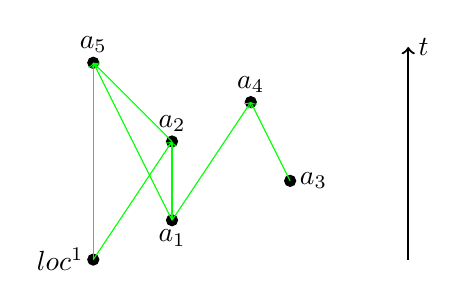
\begin{tikzpicture}
%\draw[black, thick, ->] (0,0) -- (4.5,0) node[anchor=south]{location};
\draw[black, thick, ->] (5,0) -- (5, 2.7) node[anchor=west]{$t$};

\filldraw[black] (1, 0) circle (2pt) node[anchor=east](iloc1){$loc^1$};

\filldraw[black] (2,0.5) circle (2pt) node[anchor=north](a1){$a_1$};
\filldraw[black] (2,1.5) circle (2pt) node[anchor=south](a2){$a_2$};
\filldraw[black] (3.5,1) circle (2pt) node[anchor=west](a3){$a_3$};
\filldraw[black] (3,2) circle (2pt) node[anchor=south](a4){$a_4$};
\filldraw[black] (1,2.5) circle (2pt) node[anchor=south](a5){$a_5$};

\draw[green, thin, ->] (iloc1.east) -- (a2.south);
\draw[green, thin, ->] (iloc1.east) -- (a5.south);

\draw[green, thin, ->] (a1.north) -- (a2.south);
\draw[green, thin, ->] (a1.north) -- (a4.south);
\draw[green, thin, ->] (a1.north) -- (a5.south);
\draw[green, thin, ->] (a2.south) -- (a5.south);
\draw[green, thin, ->] (a3.west) -- (a4.south);

\end{tikzpicture}
    \caption{Illustration of an example of reachability between different attack events for defender $1$.  
    For example, $next(1, 1) = \{2,4,5\}$, $next(0,1)=\{2,5\}$, $prev(2, 1) =\{0, 1\}$, $prev(1,1)=\varnothing$.
    $loc^1$ cannot reach $a_1$ since $v_1$ is not sufficiently large. For the same reason, defender $1$ cannot reach $a_3$ from $a_1$.
    }
    \label{fig:next_prev}
\end{figure}



\section{Structural Analysis}
Given that barrier forming problems studied in this work are NP-hard, a natural algorithmic choice for addressing the challenge is through exploring  mathematical programming.
%
To that end, a model must be built that selects from candidate barriers, which in turn requires the construction of a representative set of barrier candidates, a rather non-trivial task. 
%
The set of candidate barriers should satisfy two conflicting constraints: (1) it should contain a minimum set line segments that achieves the desired separation and (2) its size should not be too big that it will cripple the barrier selection process. 
%
Through careful structural analysis, we notice that the barriers to be considered can be limited to \emph{tangent} or \emph{bitangent} line segments. A tangent line segment, with respect to an object or an obstacle, is a line that passes through a vertex or an edge of the object/obstacle but does not intersect its interior. A bitangent is a line segment that is tangent to two objects and/or obstacles. 
%
This allows us to significantly reduce the number of candidates to be examined at the later selection stage.

\begin{theorem}\label{theorem:sin_tan}
For any $k$ sets of polygonal or point objects $S_1, \dots, S_k$ in the workspace $\mathcal W$, the set of line segments that are tangential to the objects and obstacles contains a set of minimum cardinality that separates $S_1, \dots, S_k$. 
\end{theorem}


\begin{proof}

% We prove that there exists a set of lines with minimum cardinality that separates $S_1, \dots, S_k$, and consists of only lines tangent to object vertices. 
Consider a set of line segments $L^*$ with minimum cardinality that separates $S_1,\dots, S_k$. 
Without loss of generality, we assume all line segments in $L^*$ do not end in the free space, i.e., each line segment in $L^*$ ends
at either object boundaries or workspace boundaries.
If some line segment in a minimum barrier is not tangent to any object vertex, denoted it as $\ell=OA$ (shown in ~\ref{fig:proof}), we show that it can be replaced by a line segment that is tangent to some object vertex. 
%
Fix one end of $\ell$, $O$ in this case, and rotate $\ell$ around $O$ in both clockwise and counterclockwise directions until it hits some object vertex and becomes tangential to the object.
%
Denote the two line segments resulting from clockwise rotation and counterclockwise rotation as $\ell_1'=OB$ and $\ell'_2=OC$, respectively. 

We show $\ell$ can be replaced with $\ell_1'$ or $\ell_2'$. 
If this is not the case,
since replacing $\ell$ with $\ell_1'$ cannot make the separation work, there must be some point $P_1$ between $AB$ that is path connected to some point in the other class without crossing any line segments in $L^*$ when $\ell$ is replaced with $\ell'_1$. Denote the point as $D_1$ and the path as $path_1$. 
The same analysis goes for $\ell'_2$, that if $\ell$ cannot be replaced by $\ell_2$ then there is some point $P_2$ in $AC$ and path $path_2$ that connects $P_2$ to some other point $D_2$ in a different class and crosses segment $\ell$ but not $\ell_2'$. 
Since there are no objects or obstacles inside triangle $OCB$, we can assume the parts of $path_1$ and $path_2$ inside triangle $OCB$ are straight lines.
So, $path_1$ and $path_2$ must cross each other at some point. 
Denote the cross point as $Q\in path_1 \cap path_2$. 
Then, $path_1 = path_{11} (from\ P_1\ to\ Q) + path_{12} (from\ Q\ to\ D_1)$ and $path_2 = path_{12} (from\ P_2\ to\ Q) + path_{22} (from\ Q\ to\ D_2)$. 
Path $p_{11} + p_{22}$ connects $P_1$ to $D_2$, and $p_{21} + p_{12}$ connects $P_2$ to $D_1$, one of which must not cross $\ell$. 
This leads to a contradiction to the fact that the original line set $L^*$ separates the $k$ classes of objects.

Therefore, each non-tangent line segment in $L^*$ can be replaced with a tangent line segment. 
It will eventually result in a set of tangent barriers with minimum cardinality that separates $S_1,\dots,S_k$.
\begin{figure}[ht]
    \vspace{-2mm}
    \centering
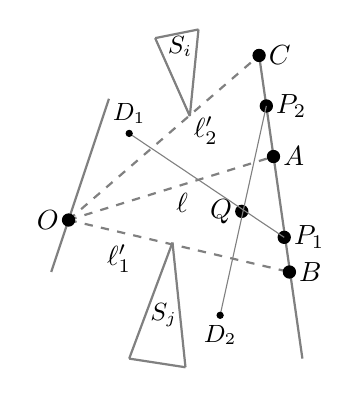
\begin{tikzpicture}[scale = 1.1]
\draw[gray, thick] (0.1, 0) -- (0.7666, 2);
\draw[gray, thick] (3, -1) -- (2.5, 2.5);


\draw[gray, thick] (1, -1) -- (1.5, 0.34);
\draw[gray, thick] (1.65, -1.1) -- (1.5, 0.34);
\draw[gray, thick] (1.65, -1.1) -- (1, -1);

\draw[gray, thick] (1.3, 2.7) -- (1.7, 1.8);
\draw[gray, thick] (1.8, 2.8) -- (1.7, 1.8);
\draw[gray, thick] (1.8, 2.8) -- (1.3, 2.7);

\draw[gray, thick, dashed] (0.3, 0.6) -- (2.66666, 1.333);

\draw[gray, thick, dashed] (0.3, 0.6) -- (2.5, 2.5);
\draw[gray, thick, dashed] (0.3, 0.6) -- (2.85, 0);

\node[text width=1cm] at (2, 0.8) {$\ell$};
\node[text width=1cm] at (2.2, 1.63) {$\ell_2'$};
\node[text width=1cm] at (1.2, 0.15) {$\ell_1'$};

\filldraw[black] (0.3, 0.6) circle (2pt) node[anchor=east] {$O$};
\filldraw[black] (2.666, 1.333) circle (2pt) node[anchor=west] {$A$};
\filldraw[black] (2.5, 2.5) circle (2pt) node[anchor=west] {$C$};
\filldraw[black] (2.85, 0) circle (2pt) node[anchor=west] {$B$};

\filldraw[black] (2.79, 0.4) circle (2pt) node[anchor=west] {$P_1$};
\filldraw[black] (2.5833, 1.917) circle (2pt) node[anchor=west] {$P_2$};

\filldraw[black] (2.3, 0.7) circle (2pt) node[anchor=east] {$Q$};

\draw[gray] (2.79, 0.4) -- (1.0, 1.6);
\draw[gray] (2.5833, 1.917) -- (2.05, -0.5);
\filldraw[black] (1.0, 1.6) circle (1pt) node[anchor=south] {\small{$D_1$}};
\filldraw[black] (2.05, -0.5) circle (1pt) node[anchor=north] {\small $D_2$};


\node[text width=1cm] at (1.9, 2.6) {\small $S_i$};
\node[text width=1cm] at (1.7, -0.5) {\small $S_j$};

\end{tikzpicture}
    \caption{Rotating non-tangent barrier line segment $\ell$ in clockwise and counterclockwise directions around its endpoint $O$ until it becomes tangential to some objects.}
    \label{fig:proof}
    \vspace{-2mm}
\end{figure}
% Then, we show that there exists a set of lines with minimum cardinality that separates $S1$ and $S2$. Similarly, when a line is only tangent to one vertex
\end{proof}

Although we can limit the candidate barriers to line segments tangent to object vertices, there can
still be infinite number of candidates. 
One may consider using line segments that are bitangent to
object vertices, i.e. line segments crossing two object or obstacle vertices. If there are $n$ object/obstacle vertices, there can be at most $n^2$, i.e., a quadratic number of bitangents. 
Unfortunately, bitangent lines are insufficient to act as candidate barriers by themselves for polygonal objects. A counterexample in ~\ref{fig:counter} shows that there is an instance where an optimal solution must contain line segments that are not bitangents. 
%
In this counterexample, we need separate the orange objects from the lime object. A minimum of three line segments are used, and it is not possible that all of them are bitangent, i.e.

\begin{proposition}
Bitangent line segments do not always contain optimal solution for the barrier forming problem for polygonal objects.
\end{proposition}

\begin{figure}[ht]
    \centering
    \vspace{-.2in}
    \includegraphics[width = .25\textwidth]{chapters/bc/fig/counter_example.png}
    \vspace{0.0in}
    \caption{Counterexample that shows using only bitangent line segments cannot create the optimal solution}
    \label{fig:counter}
\end{figure}

Despite the caveat, for the first two formulations that deal with barrier forming for point sets, even with polygonal obstacles, bitangent line segments
always contain an optimal solution. More precisely, 
\begin{theorem}
For any $k$ sets of point objects $S_1, \dots, S_k$ in a workspace $\mathcal W$, there exists
a set of line segments with minimum cardinality that separates $S_1, \dots, S_k$, 
and only consists of bitangent line segments.
\end{theorem}

\begin{proof}
From Theorem~\ref{theorem:sin_tan}, we can see using single tangent line segments is always enough
for an optimal solution. 
Now we turn an optimal solution, $L^*$, with only tangent line segments, into
a solution with only bitangent line segments while still maintaining the same number of barriers. 

For a tangent line segment $\ell=AB\in L^*$ with tangent point $O$ (shown in ~\ref{fig:proof_bi}), and if $O$ is a point object, assume it is beneath $\ell$,
rotate $\ell$ clockwise around $O$ until it hits a point object or an obstacle vertex.
Denote the resulting line segment as $\ell'$, and replace $\ell$ with $\ell'$.
Since the objects are point objects, so $BB'$ and $AA'$ must belong to obstacles or workspace boundary, 
and thus there is no object point inside $OAA'$ or $OBB'$. 
Therefore, the replacement won't result in
any path connecting objects in different classes.
If this is not the case, then there will be some path connecting two object points in different classes that crosses $\ell$ but does not cross $\ell'$ or other barriers. 
Since the triangle areas $OAA'$ and $OBB'$ are empty, that path must enter region $OAA'$ or $OBB'$ and leave them from $\ell$. Then, that part of the path could be replaced with a straight line segment parallel to $\ell$ which prevents it from crossing $\ell$. This contradicts the assumption that $L^*$ prevents all connections between objects in different classes. % of objects.

Continuing the replacement until all line segments are bitangent will result in an optimal solution with only bitangent line segments.

\begin{figure}[ht]
    \centering
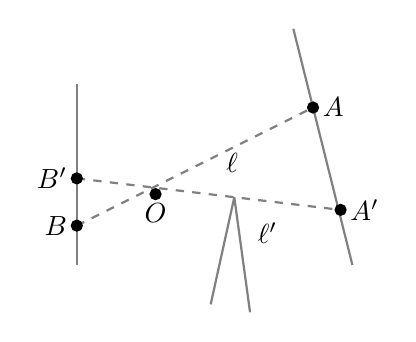
\begin{tikzpicture}
% \draw[gray, thick] (0, 0) -- (1, 2);
\draw[gray, thick] (2.5, -1) -- (1.75, 2);
\draw[gray, thick] (-1, -1) -- (-1, 1.3);

\draw[gray, thick] (0.7, -1.5) -- (1, -0.14);
\draw[gray, thick] (1.2, -1.6) -- (1, -0.14);

% \draw[gray, thick] (3, -1) -- (2.5, 2.5);

% \draw[gray, thick] (1, -1) -- (1.5, 0.34);
% \draw[gray, thick] (1.65, -1.1) -- (1.5, 0.34);
% 
% \draw[gray, thick, dashed] (0.3, 0.6) -- (2.66666, 1.333);
\draw[gray, thick, dashed] (-1., -0.5) -- (2., 1.);

\draw[gray, thick, dashed] (-1., 0.1) -- (2.35, -0.3);

% \draw[gray, thick, dashed] (0.3, 0.6) -- (2.5, 2.5);
% \draw[gray, thick, dashed] (0.3, 0.6) -- (2.85, 0);

\node[text width=1cm] at (1.4, 0.3) 
                        {$\ell$};
% \node[text] at (1.8, 1.63) 
                        % {$\ell_2'$};
\node[text width=1cm] at (1.8, -0.6) 
                        {$\ell'$};

\filldraw[black] (0.0, -0.1) circle (2pt) node[anchor=north] {$O$};
\filldraw[black] (2, 1.) circle (2pt) node[anchor=west] {$A$};
% \filldraw[black] (2.5, 2.5) circle (2pt) node[anchor=west] {$C$};
\filldraw[black] (-1, -0.5) circle (2pt) node[anchor=east] {$B$};

\filldraw[black] (2.35, -0.3) circle (2pt) node[anchor=west] {$A'$};
\filldraw[black] (-1, 0.1) circle (2pt) node[anchor=east] {$B'$};

% \filldraw[black] (2.7583, 0.6666) circle (2pt) node[anchor=west] {$P_1$};
% \filldraw[black] (2.5833, 1.917) circle (2pt) node[anchor=west] {$P_2$};

\end{tikzpicture}
    \caption{Rotating a single tangent barrier line segment $\ell$ around its tangent point $O$ clockwise until it becomes bitangent.}
    \label{fig:proof_bi}
\end{figure}
\end{proof}

For separating polygonal objects, although using bitangent line segments cannot guarantee an optimal solution that uses minimum number of line segments, they can still ensure that solutions limited to bitangents are at least $2$-optimal.
\begin{proposition}
For any $k$ sets of polygonal objects $S_1, \dots, S_k$ in the workspace $\mathcal W$, there exists a set of line segments with cardinality at most twice the minimum cardinality, that separates $S_1, \dots, S_k$, and only consists of line segments that are bitangent to object or obstacle vertices. 
\end{proposition}
\begin{proof}


\begin{figure}[ht]
    \centering
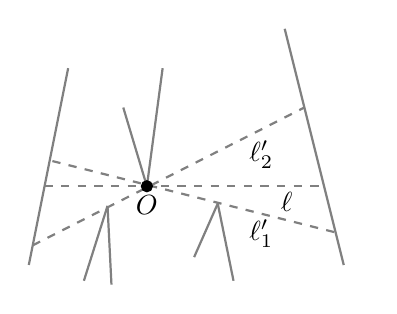
\begin{tikzpicture}

\draw[gray, thick] (2.5, -1) -- (1.75, 2);
\draw[gray, thick] (-1.5, -1) -- (-1, 1.5);
\draw[gray, thick] (0, 0) -- (-0.3, 1);
\draw[gray, thick] (0, 0) -- (.2, 1.5);

\draw[gray, thick] (-0.8, -1.2) -- (-0.5, -0.25);
\draw[gray, thick] (-0.45, -1.25) -- (-0.5, -0.25);

\draw[gray, thick] (0.6, -0.9) -- (0.9, -0.22);
\draw[gray, thick] (1.1, -1.2) -- (0.9, -0.22);


\draw[gray, thick, dashed] (-1.45, -0.75) -- (2., 1.);
\draw[gray, thick, dashed] (-1.3, -0.0) -- (2.2, 0);

\draw[gray, thick, dashed] (-1.2, 0.32) -- (2.45, -0.6);



\node[text width=1cm] at (2.2, -0.2) 
                        {$\ell$};

\node[text width=1cm] at (1.8, -0.6) 
                        {$\ell'_1$};

\node[text width=1cm] at (1.8, 0.4) 
                        {$\ell'_2$};

\filldraw[black] (0.0, -0.0) circle (2pt) node[anchor=north] {$O$};


\end{tikzpicture}
    \caption{Rotating tangent barrier line segment $\ell$ both clockwise and counterclockwise around its tangent point $O$ until it becomes bitangent.}
    \label{fig:proof_bi_2opt}
\end{figure}

Starting from an optimal solution $L^*$ with only tangent line segments,
we will replace each tangent line segment with two bitangent line segments.

Rotate each non-bitangent line segment $\ell\in L^*$ around its tangent point $O$ in clockwise or counterclockwise directions until the line segment become bitangent, as illustrated in ~\ref{fig:proof_bi_2opt}. 
Since any path connecting two objects in different classes and is cut by barrier $\ell$ will still be cut by $\ell'_1$ and $\ell'_2$.
The replacement can still guarantee the separation among the object groups.
After replacing all barriers, we can obtain a 2-OPT solution with the number of line segments twice the minimum.
\end{proof}
\label{sec:bd-structure}
\subsection{Algorithmic Solutions for \prob}\label{sec:bd-algorithm}
In this section, we describe three methods for solving infinite-horizon \prob (Problem~\ref{prob:bd-1}).
Sec.~\ref{sec:bd-dp} provide a dynamic programming (DP) algorithm based on one developed in \cite{adler2022role}, 
followed by Sec.~\ref{sec:bd-ilp} formulating an integer linear programming model,
and Sec.~\ref{sec:bd-dp_local} discusses a heuristic search algorithm based on the DP algorithm. 
The extension to an infinite attack stream with a finite look-ahead horizon  (Problem~\ref{prob:bd-2}) will be discussed in Sec.~\ref{sec:bd-hor}.


\subsection{Exact Dynamic Programming Based Method}%for A Fixed Number of Defenders}
\label{sec:bd-dp}

The DP algorithm builds a recursion formula on the last attacks intercepted by the defenders.
Without loss of generality, we assume that each attack is only intercepted by one defender.
For a DP state $a_1, \dots, a_k$ where $a_i$ is the last attack defender $i$ intercepts, 
let $T[a_1]\dots[a_k]$ store the maximum number of attacks that can be intercepted when the $i^{th}$ defender's last intercepted attack events is $a_i$ $(i\in[1,k])$,
and denote $a_{ma}$ as the maximum of $a_1, \dots, a_k$.
Base on which attack the $ma^{th}$ defender intercepts before intercepting attack $a_{ma}$,
we can write the DP recursion formula as follows.
\begin{equation}
\begin{split}
T[a_1]\dots[a_{ma}]\dots[a_k] &= \\ 
\max_{p\in prev(a_{ma}, ma) \wedge p\neq a_1 \dots a_k} &  T[a_1]\dots[p]\dots[a_k] + 1
\end{split}
\end{equation}

Pseudo-code in Alg.~\ref{alg:bd-dp} provides a sketch of a possible implementation of the dynamic programming algorithm.
Effectively implemented, the time complexity of running Alg.~\ref{alg:bd-dp} is $O( (n+1)^{k+1})$, which is polynomial when $k$, the number of defenders, is fixed.
\vspace{-2mm}

\begin{algorithm}
%\begin{small}
\DontPrintSemicolon
\KwData{
$E=\big \langle loc_i, t_i\big\rangle_{i=1}^{n}$: $n$ attack events\;
$loc^1,\dots,loc^k$: initial locations of the $k$ defenders\;
$v_1,\dots,v_k$: speeds of the $k$ defenders\;
}
\KwResult{Maximum number of attacks intercepted}
\vspace{1mm}
$T\gets$ an $(n+1)^k$-length array initialized to $-\infty$\;
\vspace{1mm}
$result\gets 0$\;
\vspace{1mm}
$T[0]\gets 0$\;
\vspace{1mm}
\For{$mask\gets 0 $ \KwTo $(n+1)^k - 1$}{
\vspace{1mm}
    $\overline{a_1 a_2\dots a_k} \leftarrow mask$\;
    \Comment{$\overline{a_1 a_2\dots a_k}$ represents a base-($n+1$) number, i.e., $a_1\cdot (n+1)^{k-1} + a_2 \cdot (n+1)^{k-2} +\dots+ a_k$}
    \If{$\exists\ a_i = a_j$}{
        \Continue\;
    }
\vspace{1mm}
    $ma \leftarrow argmax_i a_i$\;
\vspace{1mm}
    \For{$p\in prev(a_{ma}, ma)$}{
        \If{$\forall i\ pos_i \neq p$}{
            $pm\gets mask - (a_{ma} - p)\cdot (n+1)^{k-ma}$\;
            \Comment{$pm$ is the result of replacing $a_{ma}$ with $p$}
            $T[mask]\gets \max(T[mask], T[pm] + 1)$\;
        }
    }
\vspace{1mm}
    $result\gets \max(result, T[mask])$\;
}
\vspace{1mm}
\Return{$result$}\;

\caption{Dynamic Programming for \prob}
\label{alg:bd-dp}
%\end{small}
\end{algorithm}
\vspace{-2mm}
%\vspace{-15mm}

The algorithm presented here is a slight modification of the DP algorithm in \cite{adler2022role} with two subtle differences. First, we enforce that an attack event can only be handled by one defender.
Second, we explicitly use the initial locations of the defenders in the algorithm, which is essential for handling the finite horizon extension.

\subsection{Solving \prob with Integer Linear Programming Model based on a Flow Formulation}
\label{sec:bd-ilp}

It is not difficult to see that \prob can also be seen as a network flow problem by treating each attack event as a node and the reachability between each pair of attack events for each defender as the edges in the graph. 

Specifically, there are $n$ nodes in the graph, representing the $n$ attack events. 
There are also $O(n^2k)$ connections between nodes inside the graph.
If defender $j$ can reach attack event $i'$ from $i$, there is an connection 
$edge[i][i'][j]$ between node $i$ and $i'$. 
Also, we use a binary variable $intercept[i]$ to denote whether attack event $i$ is successfully intercepted. 
These give rise to the following integer linear programming (ILP) formulation of the problem.

% \begin{gather}
Eq. \eqref{eq:bd-intercept} sets the criteria of an attack $i$ being intercepted as at least one defender to come into the node $i$, which means intercept attack $i$.
Eq. \eqref{eq:bd-flow} sets the defender flow conservation rule that the number of type $j$ defender exiting node $i$ must be larger than or equal to the number of type $j$ defender coming to node $i$.
Eq. \eqref{eq:bd-initial} sets the initial constraints on the number of each type of defender used (coming out from node 0).

\begin{gather}
\sum_{j\in[1, k],\ i'\in prev(i, j)} edge[i'][i][j] \geq intercept[i] \label{eq:bd-intercept}\\
\sum_{nxt_i\in next(i, j)} edge[i][nxt_i][j] \leq \sum_{prv_i \in prev(i,j)} edge[prv_i][i][j]  \label{eq:bd-flow} \\
\sum_{nxt_0 \in next(0, j)} edge[0[nxt_0][j] \leq 1 \label{eq:bd-initial}  \\
Objective\quad \max \sum_i intercept[i]
\end{gather}

% \end{gather}
Denote $M$ as the number of connections in the graph, clearly $M<n^2k$.
This integer linear programming formulation uses $M + n$ variables, and 
$nk + n$ constraints. 

%It may not be worth mentioning
\begin{remark}
The flow formulation of the problem is an NP-hard problem. The proof is similar to the NP-completeness proof of the two-commodity flow in \cite{even1975complexity}. This seems to suggest that \prob is NP-hard as well. 
\end{remark}

% \begin{proof}
% \end{proof}

\subsection{Exhaustive Defenders Pairing Heuristic Search Method}
\label{sec:bd-dp_local}
We now develop a heuristic search method using the dynamic programming algorithm discussed in Alg.~\ref{alg:bd-dp} 
applied on two defenders.
The DP algorithm that computes the optimal solution for two defenders is used as a local improvement primitive 
for the local search heuristic algorithm. 

We call the resulting algorithm \emph{exhaustive defender pairing} (\ours).  
In each iteration, \ours pick two defenders, and the attack events the two defenders have intercepted and the attack events that have not been intercepted by any defender. 
Then, \ours uses the DP algorithm in Alg.~\ref{alg:bd-dp} to increase the number of attack events intercepted by the two defenders selected. 
The complete algorithm is sketched in Alg.~\ref{alg:bd-dp_local}.

\begin{algorithm}[h]
\DontPrintSemicolon
\KwData{
$E=\big \langle loc_i, t_i\big\rangle_{i=1}^{n}$: $n$ attack events\;
$loc^1,\dots,loc^k$: initial locations of the $k$ defenders\;
$v_1,\dots,v_k$: speeds of the $k$ defenders\;
}
\KwResult{Number of attacks intercepted}

$Intercept \gets$ a length-$n$ array initialized to $-1$\;
\Comment{$Intercept$ array stores for each event the defender that intercepts it}
$result\gets 0$\;
\vspace{1mm}
\For{$u, v \in \{1, \dots, k\}\times\{1, \dots, k\}, u\neq v$}{
    $E'\gets \{w\ |\ Intercept[w] \in\{u, v, -1\}\}$ \;
    \Comment{$E'$ stores the set of attack events intercepted by defender $u,v$ and the attacks not intercepted by any defender}
\vspace{1mm}
    $\tilde{n}\gets E'.size$\;
\vspace{1mm}
    T $\gets$ an $(\tilde{n}+1)^2$-length array initialized to $-\infty$\;
\vspace{1mm}
    $T[0]\gets 0$\;
    \Comment{Apply the DP algorithm for defender $u$ and $v$}
\vspace{1mm}
    \For{$mask\gets 0 $ \KwTo $(\tilde{n}+1)^2-1$}{
        $\overline{a_1 a_2} \leftarrow mask$\;
        \If{$a_1 =a_2$}{
            \Continue\;
        }
\vspace{1mm}
        $ma \leftarrow argmax_i a_i$\;
\vspace{1mm}
        \For{$p\in prev(a_{ma}, ma)$}{
            \If{$\forall i\ a_i \neq p$}{
                $pm\gets mask - (a_{ma} - p)\cdot (n+1)^{2-ma}$\;
                $T[mask]\gets \max(T[mask], T[pm] + 1)$\;
            }
        }
        % $result\gets \max(result, T[mask])$\;
    }
\vspace{1mm}
    \If{Solution is improved}{
        Update $Intercept, result$\;
    }
}
\vspace{1mm}
\Return{$result$}
\caption{Exhaustive Defender Pairing}
\label{alg:bd-dp_local}
\end{algorithm}

We can try different defender pairing orders and choose the best one. 
In our \ours implementation, we choose to run line 3 of Alg.~\ref{alg:bd-dp_local} in 3 different iteration ordering of $u, v$.
Alg.~\ref{alg:bd-dp_local}'s running time is $O(k^2 n^3)$ as we try $O(k^2)$ pairs of defenders, and each run of the DP algorithm takes $O(n^3)$.
% ($u$ increasing from $1$ to $k$, decreasing from $k$ to $1$, increasing from $k/2$ to $k$ after which go back to $1$ and increase to $k/2-1$). 

\subsection{Handling Infinite Attack Streams with a Finite Look-Ahead Horizon }
\label{sec:bd-hor}
For Problem~\ref{prob:bd-2} where the attacks $\big \langle loc_i, t_i\big \rangle_{i=1}^{\infty}$ may be infinite, and the look-ahead horizon is finite, not all attacks are revealed at once. As such, previous methods cannot be directly applied. 
As the future attack sequence cannot be foreseen, defenders need to \emph{react} to information (e.g., the attack events in the next $T$ time interval) obtained so far. 

Towards addressing the problem, a greedy \emph{replanning} approach can be applied. Whenever an attack event is observed, the defender team replans the capture sequence given the new attacks added to the attack queue. 
This gives rise to an online algorithm sketched in Alg.~\ref{alg:bd-horizon}.

\begin{algorithm}[h]
\DontPrintSemicolon
\KwData{
$E=\big \langle loc_i, t_i\big\rangle_{i=1}^{\infty}$: a stream of attack events\;
$loc^1,\dots,loc^k$: initial locations of the $k$ defenders\;
$v_1,\dots,v_k$: speeds of the $k$ defenders\;
}
$E'\gets $ an empty queue\;
\Comment{$E'$ stores attack events seen so far}
\vspace{1mm}
\While{new attack events added to $E'$ }{
    Apply Alg.~\ref{alg:bd-dp_local} to compute a plan for the defenders and attack events $E'$\;
    Execute the plan, pop out from $E'$ attack events passed, and update $loc^1,\dots,loc^k$ to the defenders' current locations until new attacks are foreseen\;
}
% \KwResult{Number of attacks intercepted}

% $Intercept \gets$ a length-$n$ array initialized to $-1$\;
% \Comment{$Intercept$ array stores for each event the defender that intercepts it}
% $result\gets 0$\;
% \For{$u, v \in \{1, \dots, k\}\times\{1, \dots, k\}, u\neq v$}{
%     $E'\gets \{w\ |\ Intercept[w] \in\{u, v, -1\}\}$ \;
%     \Comment{$E'$ stores the set of attack events intercepted by defender $u,v$ and the attacks not intercepted by any defender}
%     $\tilde{n}\gets E'.size$\;
%     T $\gets$ an $(\tilde{n}+1)^2$-length array initialized to $-\infty$\;
%     $T[0]\gets 0$\;
%     \For{$mask\gets 0 $ \KwTo $(\tilde{n}+1)^2-1$}{
%         $\overline{a_1 a_2} \leftarrow mask$\;
%         \If{$pos_0 = pos_1$}{
%             \Continue\;
%         }
%         $ma \leftarrow argmax_i pos_i$\;
%         \For{$p\in prev(a_{ma}, ma)$}{
%             \If{$\forall i\ pos_i \neq p$}{
%                 $T[mask]\gets \max(T[mask], 1 + T[\overline{a_1\dots p \dots a_k}])$\;
%             }
%         }
%         % $result\gets \max(result, T[mask])$\;
%     }
%     \If{Solution is improved}{
%         Update $Intercept, result$\;
%     }
% }
% \Return{$result$}
\caption{Online Exhaustive Defender Pairing}
\label{alg:bd-horizon}
\end{algorithm}
\subsection{Evaluation and Empirical Study of \prob}\label{sec:bd-evaluation}
For each of Problems~\ref{p:surf-1}-\ref{p:surf-3}, extensive experimental evaluations were carried out to evaluate our proposed algorithmic solutions. Here, we present representative evaluation demonstrating the effectiveness of our methods, with a focus on three realistic settings (the ICU model from ~\ref{fig:surf-ex}, bus and subway car models shown in ~\ref{fig:surf-bus-subway}). %
For all environments, the surface $S$ is selected to be all visible surfaces not facing downward.
Due to limited space, result on the (2+$\varepsilon$)-approximation algorithm (Algorithm~\ref{alg:surf-greedy}) is omitted (as shown in \cite{fengyu2020optimally}, such methods are fast but are quite sub-optimal). The experiments were carried out on a median-end quad-core Intel i7 processor with 16GiB RAM. 
Algorithms were implemented in C++. Gurobi \cite{optimization2019gurobi} was used as the Integer Programming solver. 
Source code is available at 
{\small \url{https://github.com/rutgers-arc-lab/3d_coverage}}.

\begin{figure}[!ht]
    \centering
    \includegraphics[width = .4\columnwidth]{chapters/surf/fig/bus.png}\hspace{3mm}
    \includegraphics[width = .4\columnwidth]{chapters/surf/fig/subway.png}
    \caption[Real 3D environments used in our evaluation in addition to the ICU model]
    {Realistic 3D environments used in our evaluation in addition to the ICU model from ~\ref{fig:surf-ex}. [left] A 40-foot large bus model and its interior. [right] A subway car and its interior.}
    \label{fig:surf-bus-subway}
\end{figure}

Results on Problem~\ref{p:surf-1}, using ILP, is given in ~\ref{fig:surf-coverage-ratio-vis}. 
For each model, $600$ candidate sensor locations and $20,000$ coverage surface points are sampled using grids. 
As expected, the surface coverage ratios increase as the number of sensors increase, approaching full coverage. We note that certain surface region is not visible, e.g., ground underneath seats in subway cars, leading to plateaus below $100\%$ coverage. The computation time is very reasonable for offline computations. The spikes in the middle of the computation time plot correspond to hard cases when the visibility coverage is about to plateau. We also observe that subway $<$ ICU $<$ bus in terms 
of computation time, which may be explained by the interior complexity of these environments. This aspect is different across the three problems.

\begin{figure}[!ht]
\vspace{1mm}
    \centering
    \includegraphics[width=0.475\columnwidth, height=2in]{chapters/surf/fig/result-coverage-ratio-eps-converted-to.pdf}
    \includegraphics[width=0.49\columnwidth, height=2in]{chapters/surf/fig/result-time-eps-converted-to.pdf}
    \caption[Coverage quality and computation time for Problem~\ref{p:surf-1}]
    {Coverage quality and computation time for Problem~\ref{p:surf-1} for the three environments as the number of sensors change.}
    \label{fig:surf-coverage-ratio-vis}

\end{figure}

\begin{wrapfigure}[7]{r}{1.1in}
  \vspace*{0mm}
  \begin{overpic}[width=1.1in,tics=5]{chapters/surf/fig/terrain-8.png}
	\end{overpic}
\vspace*{-6.5mm}
\end{wrapfigure}
In evaluating Problem~\ref{p:surf-2}, we first examine a case where mobile sensors
(e.g., camera drones) are deployed to cover a synthetic terrain with relatively 
small curvature, i.e., $vis(\cdot, \cdot) \equiv 1$. An illustration of the 
setting is given in the figure on the right, where the color indicates the height 
of the terrain. The sensors (8 red triangles in the figure) are placed
at a fixed height above the terrain and must guard the region enclosed 
in the black curve. Spherical range sensing is assumed. For the setup 
($600$ sensor locations and $20,000$ surface points), computation time 
and solution quality as the number of sensors changes are listed in the table. 
Computation time decreases as the number of sensors 
increases, indicating the problem is harder when sensors are too few to provide 
a good coverage. It also shows that the ILP running time does not depend positively
on sensor quantity. The quality (smaller is better) increase becomes minimal
as sensor quantity reaches $10$. 


\vspace{1mm}
\begin{table}[!ht]
    \centering
    \begin{tabular}{|c|c|c|c|c|c|c|c|c|}
    \hline
        \#Sensors   & 2     &  4    & 6      & 8     & 10    & 12    & 14    & 16 \\
        \hline
        Time (s)    & 42.9   &  25.4    & 18.5  & 12.7 & 13.1  & 11.3  & 7.64 & 6.70 \\ 
        \hline
        Radius  & 5.10     &  3.31    & 2.76      & 2.43     & 2.27    & 2.16    & 2.07    & 1.99 \\
        \hline
    \end{tabular}
    %\caption{Computation time and minimum radius for the problem 2 without visibility issue computed on a randomly generated terrain.}
    \label{tab:Terrain}
\end{table}

In a second evaluation of Problem~\ref{p:surf-2}, visibility is considered with the 
optimization coverage ratio set to $80\%$. That is, at least $80\%$ of the
maximum visible target surface (for a given $k$) will be guaranteed the achieved coverage 
quality. The result, summarized in ~\ref{fig:surf-coverage-ratio-mq}, again 
demonstrates a negative correlation between the computational time and the number 
of sensors. Here, however, the computational time is $20+$ times  more 
than when having full visibility.

\begin{figure}[!ht]
    \centering
    \includegraphics[width=.46\columnwidth, height=2in]{chapters/surf/fig/result-radius-mq-eps-converted-to.pdf}
    \includegraphics[width=.46\columnwidth, height=2in]{chapters/surf/fig/result-time-mq-eps-converted-to.pdf}
    \caption{Coverage quality (lower is better) and computation time for Problem~\ref{p:surf-2}
    for the three environments, as sensors increase.}
    \label{fig:surf-coverage-ratio-mq}
\end{figure}

Our last benchmark on Problem~\ref{p:surf-2} tests the effectiveness of the local improvement following the resolution of a coarsely generated ILP, at $60$ candidate sensor locations and $1000$ surface samples (~\ref{fig:surf-coverage-ratio-cu}). The right figure shows much faster computation time. The left figure shows that the  faster method does a decent job for the bus environment (other environments have similar outcomes). The result suggests which method to use would depend on whether computational time or solution optimality is more important to the task at hand. We note that the local improvement method does not help improve the ILP result at the higher resolution. 

\begin{figure}[!ht]
    \centering
    \includegraphics[width=.46\columnwidth, height=2in]{chapters/surf/fig/result-bus-mq-eps-converted-to.pdf}
    \includegraphics[width=.46\columnwidth, height=2in]{chapters/surf/fig/result-time-mq-coarse-eps-converted-to.pdf}    
    \caption[Solution quality and computation time for ILP + lcoal improvement on the bus environment]
    { [left] Solution quality (lower is better) for the bus environment. 
    The first curve (Bus) is the same as that from ~\ref{fig:surf-coverage-ratio-mq}. 
    [right] Computation time using coarse ILP + local improvement.}
\label{fig:surf-coverage-ratio-cu}
\end{figure}

For Problem~\ref{p:surf-3}, computation becomes more demanding. At the specified 
discretization level, most ILP models did not complete the optimization process 
in $10$ minutes. The intermediate quality result is given in ~\ref{fig:surf-computation-time-3}, on the left (the same threshold, selected to make the computation challenging, is used for all three environments), where the lines 
corresponds to the coverage ratio returned by the ILP model and the attached vertical bars show the reported optimality gap. The crosses show the updated ratio after local improvement is carried out (the triangles will be explained shortly). 
The subway data was shifted to the left to improve readability.
For the bus, we see that the local improvement does help improve solution optimality, suggesting it is the most difficult problem. For the other two, it appears that the solution by the ILP model is already quite optimal, but the ILP solver still needs time to close the gap from the above. The subway case has worse coverage by the same number of sensors because it is larger. If we run a coarse ILP model ($60$ sensor candidates, $1000$ surface sample) for one minute and then do local improvement, we get coverage ratios shown as the triangles in ~\ref{fig:surf-computation-time-3}, left. ~\ref{fig:surf-computation-time-3}, right shows the total computation time used. We observe that except for the challenging bus model, the faster method achieves essentially identical optimality as running ILP at higher resolutions. Subway costs most time here because it is the largest. 

\begin{figure}[!ht]
    \centering
    \includegraphics[width=.48\columnwidth, height=2in]{chapters/surf/fig/result-coverage-ratio-3-eps-converted-to.pdf}
    \includegraphics[width=.48\columnwidth, height=2in]{chapters/surf/fig/result-time-3-coarse-eps-converted-to.pdf}
    \caption[Computation time for Problem~\ref{p:surf-3}]{[left] Coverage ratio (lines) for Problem~\ref{p:surf-3} returned by multiple methods. [right] Computation time used by running a coarse ILP plus local improvements.}
    \label{fig:surf-computation-time-3}
\end{figure}

% For the last evaluation of Problem~\ref{p:3}, 

Lastly, we provide some additional visualization to help further demonstrate the structure of the problems. ~\ref{fig:surf-icu-comp} shows that Problems~\ref{p:surf-2} and~\ref{p:surf-3} induce different optimal distribution of sensors. Generally, Problems~\ref{p:surf-2} tends to cause the sensors to be evenly spaced out. On the other hand, Problem~\ref{p:surf-3} tends to balance between spacing out sensors and provide good cumulative coverage, which may require sensors to aggregate, which can be observed in ~\ref{fig:surf-bus}.

\begin{figure}[!ht]
\vspace{1mm}
    \centering
    \includegraphics[width = 0.35\columnwidth, height=2in]{chapters/surf/fig/icu-2-4.png}\hspace{3mm}
    \includegraphics[width = 0.35\columnwidth, height=2in]{chapters/surf/fig/icu-3-4.png}
\vspace{1mm}
    \caption{$4$ sensor ICU result for Problems~\ref{p:surf-2} (left) and~\ref{p:surf-3}(right).}
    \label{fig:surf-icu-comp}
\end{figure}

\begin{figure}[!ht]
\vspace{-1mm}
    \centering
    \includegraphics[width = .25\columnwidth]{chapters/surf/fig/illustration_bus.png}
    \includegraphics[width = .23\columnwidth]{chapters/surf/fig/bus-3-3.png}
    \includegraphics[width = .23\columnwidth]{chapters/surf/fig/bus-3-4.png}
    \includegraphics[width = .23\columnwidth]{chapters/surf/fig/bus-3-5.png}
    \caption[The coverage of bus]{The coverage of bus (see through model on the left) using $3$ to $5$ sensors under Problem~\ref{p:surf-3}. Aggregation of sensors at the front of the bus, which is structurally more complex, can be observed. }
    \label{fig:surf-bus}
\end{figure}



%\begin{figure}[!ht]
%    \centering
%    \vspace{-0.5in}
%    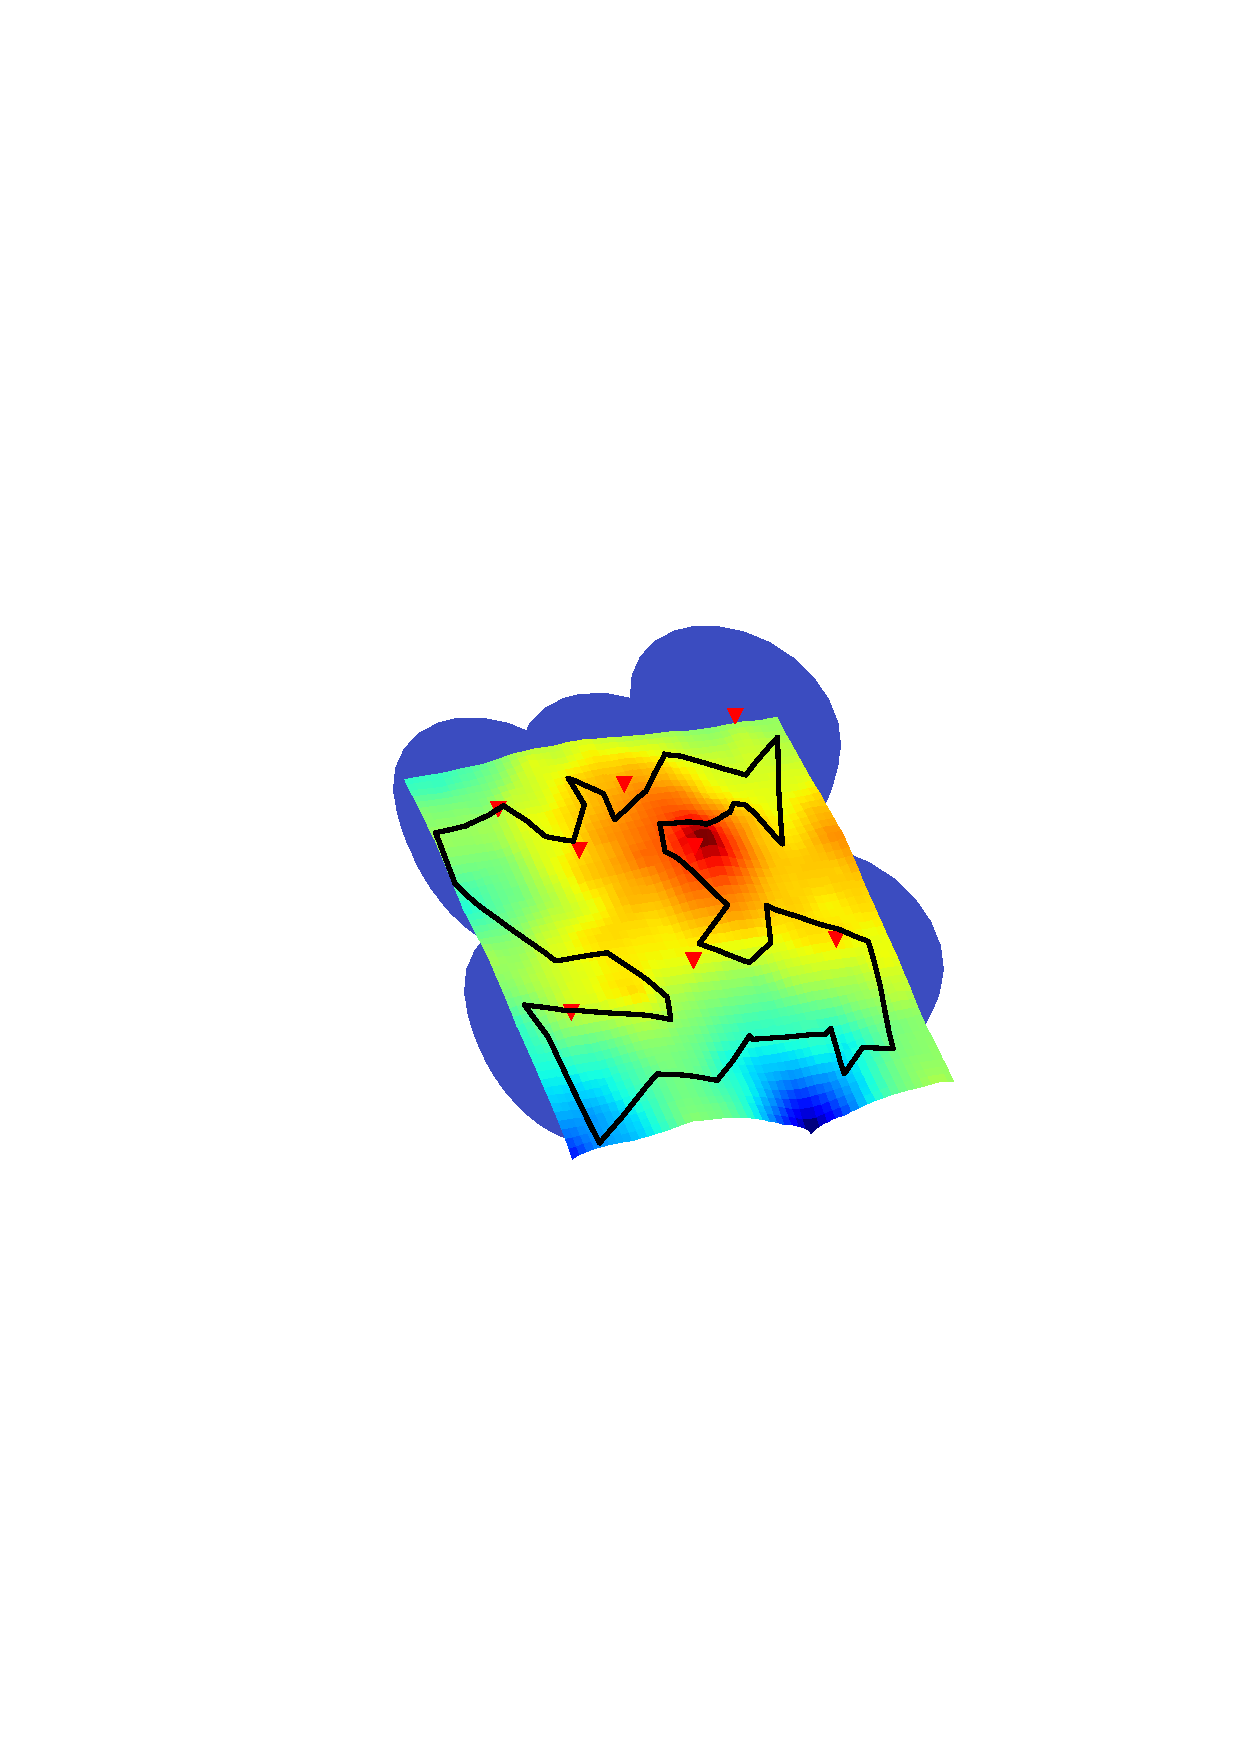
\includegraphics[width=\columnwidth, height=1.65in]{fig/terrain_8_spheres.png}
%    \vspace{-0.5in}
%    \caption{Covering a randomly generated terrain region (enclosed in black lines) with %8 sensors, for Problem~\ref{p:2}.}
%    \label{fig:terrain_8_spheres}
%\end{figure}

%% Coverage quality - # sensor curve for visibility model
% \begin{comment}
% Experiment data:
% Visibility:

% ICU computation time
% 161.070609 151.295530 330.685622 557.836444 429.295166 297.618731 304.730803 440.795053
% Coverage out of 20000
% 14082 17622 18588 18975 19252 19445 19535 19608

% Train computation time
% 33.274342 34.031417 37.465971 235.116101 202.418864 91.999594 28.336419 26.826848
% Coverage out of 20000
% 13549 16903 18557 19250 19492 19704 19811 19856

% Bus computation time
% 82.551965 47.326792 49.360691 819.235458 1155.414985 843.010299 301.578288 292.435206
% Coverage out of 20000
% 10874 13896 15788 17047 17791 18254 18626 18855


% Cumulative quality:
% ICU objective gap after 10 mins
% 0 0.137288 0.078094 0.061441 0.046752 0.033730 0.040505 0.026052
% Coverage out of 10000
% 3421 6592 7683 8203 8513 8746 8789 8982

% Train:
% ICU objective gap after 10 mins
% 0 0.279252 0.275232 0.271503 0.263170 0.251072 0.227925 0.186125
% Coverage out of 10000
% 1025 2299 3230 3860 4404 4899 5436 5910

% Bus:
% Bus objective gap after 10 mins:
% 0 0.219363 0.104556 0.086342 0.065497 0.049472 0.043567 0.034721
% Coverage out of 10000
% 1897 3770 5356 6231 7008 7479 7827 8122
% \end{comment}

% 

% Coverage quality maximization
% Coverage quality - cumulative







% \begin{comment}
% % cone model
% \begin{table}[!ht]
%     \centering
%     \begin{tabular}{|c|c|c|c|c|c|c|c|c|}
%     \hline
%         \#sensors   & 2     &  4    & 8     & 10    & 12    & 14    & 16 \\
%         \hline
%         Time (s)    & 25.8  &  23.9 & 14.1  & 14.3  & 15.3  & 13.3  & 13.8\\ 
%         \hline
%         Cone Angle  &  60.4 &  47.5 & 33.5  & 30.9  & 28.7  & 25.6  & 24.1\\
%         \hline
%     \end{tabular}
%     \caption{Computation time and minimum cone angle for the cone model computed on a randomly generated terrain.}
%     \label{tab:Terrain}
% \end{table}
% \end{comment}




%% The visibility and cumulative exposure model's visualization

\begin{comment}
\begin{figure}[!ht]
    \centering
    % \includegraphics[width=0.49\columnwidth]{fig/icu_sampled.png}
    \includegraphics[width=0.49\columnwidth]{fig/icu_result.png}
    \includegraphics[width=0.49\columnwidth]{fig/icu_result_3.png}
    % 73965/ 78549
    
    % \includegraphics[width=0.52\columnwidth]{fig/train_sampled.png}
    \hspace{-0.1in}
    \includegraphics[width=0.54\columnwidth]{fig/train_result.png} 
    \hspace{-0.4in}
    \includegraphics[width=0.54\columnwidth]{fig/train_result_3.png}
    % 14160 / 19604
    
    %\includegraphics[width=0.52\columnwidth]{fig/bus_original.png}
    % \includegraphics[width=0.52\columnwidth]{fig/bus_sampled.png}
    % \hspace{-0.3in}
    \includegraphics[width=0.52\columnwidth]{fig/bus_result.png} 
    \hspace{-0.3in}
    \includegraphics[width=0.52\columnwidth]{fig/bus_result_3.png} 
    % 45148 / 54229
    {
    \small{
    \caption{The illustration of the the results of coverage of the ICU, train and bus meshes using the visibility model and the cumulative exposure model using 4 sensors. 
    The coverage ratios are 94.2\%, 72.2\%, 83.2\%, for the visibility model, respectively. 
    The coverage ratios are 82.0\%, 38.6\%, 62.31\%, for the cumulative exposure model, respectively. 
    }
    }
    }
    \label{fig:my_label}
\end{figure}

\begin{figure}
    \centering
    \includegraphics[width = .31\columnwidth]{fig/illustration_bus.png}
    \includegraphics[width = .31\columnwidth]{fig/illustration_bus_mq_1.png}
    \includegraphics[width = .31\columnwidth]{fig/illustration_bus_mq_2.png}
    \includegraphics[width = .31\columnwidth]{fig/illustration_bus_mq_3.png}
    \includegraphics[width = .31\columnwidth]{fig/illustration_bus_mq_4.png}
    \includegraphics[width = .31\columnwidth]{fig/illustration_bus_mq_5.png}
    \caption{The coverage of the bus model using $1$ to $5$ lights with the maximum quality model.}
    \label{fig:my_label}
\end{figure}
\end{comment}

%% Comparison with different number of sensors problem 2


%% Comparison with different number of sensors

\subsection{Conclusion}\label{sec:bd-conclusion}
This paper studied the heterogeneous perimeter defense problem, as formulated in \cite{adler2022role}, with the aim of
significantly boosting the scalability to work on many defenders while achieving high levels of solution optimality.
Toward achieving this goal, we developed an exact integer programming-based algorithm with better scalability than the original dynamic programming (DP) based algorithm from \cite{adler2022role}. We then further developed a fast and highly-effective heuristic based on the pairwise application of DP for computing near-optimal solutions, scaling to dozens of defenders.
%
This pairwise application of DP is of independent algorithmic interest. 
%
In addition, we extend our solution to a more realistic online version in which only attackers within a finite time window are visible. 
%
The algorithms are thoroughly evaluated on a diverse set of boundary topologies including circles, intervals, spheres, and squares. 
%
The evaluation not only confirms that \ours is highly effective but clearly demonstrates the benefit of employing heterogeneous defenders. 